%%%%%%%%%%%%%%%%%%%%%%%%%%%%%%%%%%%%%%%%%%%%%%%%%%%%%%%%%%%%%%%%%%%%%%%%%%%%
% AGUJournalTemplate.tex: this template file is for articles formatted with LaTeX
%
% This file includes commands and instructions
% given in the order necessary to produce a final output that will
% satisfy AGU requirements, including customized APA reference formatting.
%
% You may copy this file and give it your
% article name, and enter your text.
%
%
% Step 1: Set the \documentclass
%
%

%% To submit your paper:
%\documentclass[draft]{agujournal2019}
%\usepackage{url} 
%\usepackage{graphicx,natbib,overpic,xcolor}
%\usepackage{apacite}
%\bibliographystyle{unsrtnat}
%this package should fix any errors with URLs in refs.
%\usepackage{lineno}
%\usepackage{geometry}
%\usepackage[table,xcdraw]{xcolor}
%\usepackage[inline]{trackchanges} %for better track changes. finalnew option will compile document with changes incorporated.
%\usepackage{soul}
%\linenumbers

\documentclass[draft,linenumbers]{agujournal2019}
\usepackage{tikz}
\usepackage{apacite}
\usepackage{url} %this package should fix any errors with URLs in refs.
\usepackage{enumitem}
\usepackage{amsmath}
\usepackage{overpic}
\usepackage{pict2e}
\usepackage{picture}
\usepackage{bm}
%%%%%%%

\draftfalse
\def\Var{{\textrm{Var}}\,}
%% Enter journal name below.
%% Choose from this list of Journals:
%
% JGR: Atmospheres
% JGR: Biogeosciences
% JGR: Earth Surface
% JGR: Oceans
% JGR: Planets
% JGR: Solid Earth
% JGR: Space Physics
% Global Biogeochemical Cycles
% Geophysical Research Letters
% Paleoceanography and Paleoclimatology
% Radio Science
% Reviews of Geophysics
% Tectonics
% Space Weather
% Water Resources Research
% Geochemistry, Geophysics, Geosystems
% Journal of Advances in Modeling Earth Systems (JAMES)
% Earth's Future
% Earth and Space Science
% Geohealth
%
% ie, \journalname{Water Resources Research}

\journalname{Nature Geoscience}

\begin{document}

%% ------------------------------------------------------------------------ %%
% Title
%
% (A title should be specific, informative, and brief. Use
% abbreviations only if they are defined in the abstract. Titles that
% start with general keywords then specific terms are optimized in
% searches)
%
%% ------------------------------------------------------------------------ %%

% Example: \title{This is a test title}

\title{Diurnal Self-Aggregation}

%% ------------------------------------------------------------------------ %%
%
% AUTHORS AND AFFILIATIONS
%
%% ------------------------------------------------------------------------ %%

% Authors are individuals who have significantly contributed to the
% research and preparation of the article. Group authors are allowed, if
% each author in the group is separately identified in an appendix.)

% List authors by first name or initial followed by last name and
% separated by commas. Use \affil{} to number affiliations, and
% \thanks{} for author notes.
% Additional author notes should be indicated with \thanks{} (for
% example, for current addresses).

% Example: \authors{A. B. Author\affil{1}\thanks{Current address, Antartica}, B. C. Author\affil{2,3}, and D. E.
% Author\affil{3,4}\thanks{Also funded by Monsanto.}}

\authors{Jan O. Haerter}


% \affiliation{1}{First Affiliation}
% \affiliation{2}{Second Affiliation}
% \affiliation{3}{Third Affiliation}
% \affiliation{4}{Fourth Affiliation}

\affiliation{1}{Niels Bohr Institute, University of Copenhagen, Blegdamsvej 17, 2100 Copenhagen, Denmark}
%(repeat as many times as is necessary)

%% Corresponding Author:
% Corresponding author mailing address and e-mail address:

% (include name and email addresses of the corresponding author. More
% than one corresponding author is allowed in this LaTeX file and for
% publication; but only one corresponding author is allowed in our
% editorial system.)

% Example: \correspondingauthor{First and Last Name}{email@address.edu}

\correspondingauthor{Jan O. Haerter}{haerter@nbi.ku.dk}

%% Keypoints, final entry on title page.

% List up to three key points (at least one is required)
% Key Points summarize the main points and conclusions of the article
% Each must be 100 characters or less with no special characters or punctuation and must be complete sentences

% Example:
% \begin{keypoints}
% \item	List up to three key points (at least one is required)
% \item	Key Points summarize the main points and conclusions of the article
% \item	Each must be 100 characters or less with no special characters or punctuation and must be complete sentences
% \end{keypoints}

%\begin{keypoints}
%\item Self-aggregation is possible within short timeperiods, when boundary conditions oscillate,
%\item the effect is nearly independent of domain size or resolution,
%\item the effect requires only moderate temperature amplitudes.
%\end{keypoints}

%% ------------------------------------------------------------------------ %%
%
% ABSTRACT and PLAIN LANGUAGE SUMMARY
%
% A good Abstract will begin with a short description of the problem
% being addressed, briefly describe the new data or analyses, then
% briefly states the main conclusion(s) and how they are supported and
% uncertainties.

% The Plain Language Summary should be written for a broad audience,
% including journalists and the science-interested public, that will not have 
% a background in your field.
%
% A Plain Language Summary is required in GRL, JGR: Planets, JGR: Biogeosciences,
% JGR: Oceans, G-Cubed, Reviews of Geophysics, and JAMES.
% see http://sharingscience.agu.org/creating-plain-language-summary/)
%
%% ------------------------------------------------------------------------ %%

%% \begin{abstract} starts the second page

%\begin{abstract}
\noindent
{\bf
Convective self-aggregation is a paradigm for tropical oceanic cloud organization and gives rise to cloud clusters over timescales of weeks. While much is known from standard radiative-convective equilibrium (RCE) setup with constant surface temperature, it remains poorly understood how diurnally oscillating surface temperature affects the clustering of rain events. 
By processing convection-resolving simulations with oscillating surface temperature, we find the atmosphere to equilibrate at the system scale and domain-averaged precipitation to become similar from day to day. However, the spatial distribution of precipitation is only homogeneous during the first day. 
From the second day on we find, the precipitation field is strongly structured and continues to cluster in subsequent days.
We show that the clustering is robust to changes in resolution, domain size, and surface temperature, but can be removed by reduction of the amplitude of oscillation, suggesting a transition to self-organization. Maximal clustering occurs at scales of $\mathbf{l_{max}\approx 150\;km}$, a scale we relate to the emergence of mesoscale convective systems. 
At $\mathbf{l_{max}}$, extreme events are strongly enhanced and far exceeds the rainfall expected at random. 
We explain the transition to clustering using a simple conceptual model, which describes periodic redistribution of moisture. 
These results may help clarify, how continental extremes build up and how cloud clustering over the tropical ocean could arise much more rapidly than through conventional self-aggregation alone.
}
%{\bf Convective self-aggregation is a paradigm for tropical oceanic cloud organization \cite{wing2017convective} and gives rise to cloud clusters over timescales of weeks \cite{khairoutdinov2010aggregation,muller2012detailed}.
%In contrast to the standard radiative-convective equilibrium setup \cite{held1993radiative,tompkins1998radiative}, where surface temperature is held constant, we here allow surface temperature to oscillate diurnally.
%, leading to a repetitive synoptic state, termed perpetual equilibrium \cite{schlemmer2011diurnal,haerter2018intensified}.
%While the atmosphere gradually equilibrates at the system scale and domain-averaged precipitation indeed becomes similar from day to day, the spatial distribution of precipitation is only homogeneous during the first day. 
%From the second day on, the precipitation field is strongly structured and continues to cluster in subsequent days.
%The clustering is robust to changes in resolution, domain size, and surface temperature, but can be removed by reduction of the amplitude of oscillation, suggesting a transition to self-organization.
%Maximal clustering occurs at scales of $\mathbf{l_{max}\approx 150\;km}$, a scale we relate to the emergence of multicellular convection.
%At $\mathbf{l_{max}}$, extreme events are strongly enhanced and far exceed the rainfall expected at random.
%We explain the transition to clustering using a simple conceptual model, which describes periodic redistribution of moisture. 
%The results may help clarify, how extremes build up in mid-latitudes and how cloud clustering in the tropics could arise much more rapidly than through conventional self-aggregation alone.
%}
%\end{abstract}

%\section{Introduction}\label{sec:intro}
\noindent
General circulation models (GCMs) currently cannot simulate organized deep convection, as GCMs describe convection as a collection of non-interacting plumes, yet, the strongest observed increases in tropical convective rainfall stem from organized thunderstorms \cite{tan2015increases}. 
As a model paradigm of tropical oceanic convective clustering, self-aggregation
%, where the cloud field segregates into cloudy and less cloudy sub-domains, 
usually employs the RCE \cite{held1993radiative,tompkins1998radiative} assuming spatially and temporally constant surface temperature ($\sim 300\;K$) and insolation, and organization takes place in the course of typically several weeks \cite{bretherton2005energy,khairoutdinov2010aggregation,muller2012detailed,wing2017convective}. 
Radiation feedbacks have emerged as the "smoking gun" for sustaining and increasing clustering \cite{bretherton2005energy}, but factors such as sea surface feedbacks \cite{hohenegger2016coupled}, domain size, geometry, and resolution \cite{muller2015favors}, as well as cold pool effects \cite{jeevanjee2013convective,haerter2019convective}, all contribute.
%It has been argued, that cloudy regions --- which benefit from warming cloud feedbacks --- tend to emit less heat to space than do cloud-free regions.
%Together, these two effects induce net near-surface divergence from cloud-free regions and convergence into already cloudy ones --- bringing more moisture into cloudy regions, thus further enhancing the imbalance.

%Whereas numerical simulations often assume constant insolation as well as surface boundary conditions,
Assuming constant boundary conditions is an elegant model simplification, but especially under weak surface wind conditions and strong insolation SST amplitudes were observed to exceed five Kelvin and were suggested to modify atmospheric properties \cite{kawai2007diurnal} --- potentially even affecting the Madden-Julian Oscillation (MJO) and the El Ni\~no phenomenon.
Buoy-based instruments measure diurnal variations in tropical sea surface temperature by typically 0.5-2 Kelvin \cite{weller1996surface,johnson1999trimodal} and satellite observations detect a diurnal cycle in cloud height for the MJO \cite{suzuki2009diurnal,tian2006modulation}.
Diurnally varying precipitation intensity also emerges from numerical simulations where variations in insolation are accounted for \cite{liu1998numerical}. 
%This and earlier studies\cite{chen1997diurnal} also describe a persistent organized state of a mesoscale convective system, with characteristics of a squall line.
\cite{chen1997diurnal} describe a dynamics referred to as "diurnal dancing", where long-lived mesoscale convective systems (MCS), that is, complexes of thunderstorms spanning $100\;km$ in diameter or more, give rise to long-lasting cold pools \cite{moeng1995atmospheric} and excite bi-diurnal oscillation of local cloudiness.

Over continental regions, clustering of convection is more directly relevant for humans, as severe storms from MCS can lead to intense downdrafts and flash flooding
\cite{doswell2001severe,smith2001extreme,cintineo2013predictability}.
The continental diurnal cycle typically features a build-up of convective available potential energy during the morning hours and its release in terms of precipitation during the afternoon or evening \cite{yang2001diurnal,guichard2004modelling,brown2002large,petch2002impact,schlemmer2011diurnal,moseley2016intensification,haerter2018intensified}.
Yet, as the focus was often on the timing or the overall intensity of rainfall, simulated domains were often chosen to be relatively small and model resolutions relatively high. 
State-of-the-art regional climate models now simulate relatively large domains ($\sim 1000$ $km$ at $1$ or $2$ $\;km$ resolution), but include the full complexity of realistic boundaries \cite{ban2015heavy,prein2017simulating,rasp2018variability}.

%Sahelian MCS \cite{mathon2001life}
%Sea surface impact atmosphere \cite{kawai2007diurnal}
%2day equatorial waves \cite{haertel2004dynamics}
%scale interaction MJO diurnal cycle \cite{peatman2014propagation}
%tropical precipitation extremes and mesoscale systems \cite{rossow2013tropical}
%Rich gets richer effect \cite{chou2009evaluating}.
%Regular vs. clustered \cite{tompkins2017organization}.
We here study multi-day clustering in the thunderstorm rain field, and show, using a suite of mesoscale cloud-resolving simulations, that a transition between an unorganized to a strongly-organized state occurs, when surface temperature amplitude is sufficiently increased. 
We show that, in the latter case, clustering continues to increase from day to day --- a finding we explore and explain using conceptual modeling.
We discuss the relevance for the emergence of extreme rainfall over land and the potential impact on organized convection over the tropical ocean.

\section*{Results}\label{sec:results}
\noindent
We carry out a suite of numerical experiments on mesoscale model domains of up to $960\;km\;\times\;960\;km$ and horizontal grid resolutions of at least $1\;km$, which we supplement by sensitivity experiments regarding grid resolution, domain size, microphysics and surface conditions ({\it Details:} Materials and Methods).
We contrast simulations with different amplitudes $T_a$ but equal average surface temperature and refer to experiments with $T_a=2\;K$, $T_a=3.5\;K$ and $5\;K$ as A2, A3.5 and A5, respectively.
Each numerical experiment is run for several days, allowing for a spin-up and quasi steady-state period (Tab.~\ref{tab:experiments} and Fig.~\ref{fig:multi-day_timeseries}). 

\noindent
{\bf Domain mean time-series.}
Unsurprisingly, the differences in surface temperature amplitudes are reflected in larger amplitudes of near-surface temperatures, $T_{50\;m}$ (Fig.~\ref{fig:daily_mean}a and Fig.~\ref{fig:multi-day_timeseries}), but only modest changes to the mean $\overline{T_{50\;m}}$.
Modifications in the time-series of domain-mean rain are more profound, with $A5$ yielding a relatively sharp mid-afternoon single-peak structure, which transitions to a broader and double-peaked structure as $T_a$ is reduced (Fig.~\ref{fig:daily_mean}b) --- approaching the diurnal cycle typical of oceanic convection \cite{yang2001diurnal}.
Again, the differences in the temporal mean (dashed lines) are very small, reflecting radiation constraints on rainfall \cite{held2006robust}.
Approximately proportional curves are found for rain area fraction, which however differs from those of rain rate immediately before the main peak in rate (Fig.~\ref{fig:daily_mean}c).
These differences are made more transparent when inspecting rain rates conditional on a threshold ($I>I_0$ with $I_0=.5\;mm\;h^{-1}$, Fig.~\ref{fig:daily_mean}d). 
Both mean and heavy precipitation show a pronounced evening peak for $A5$ and an early-morning peak for $A2$.
In summary, whereas time averages are nearly identical for numerical experiments with varying forcing amplitude, the time-series of rain rate differ markedly.
Time-averaged free tropospheric temperatures, which constrain the rate of radiative emission and thereby overall rain rate \cite{held2006robust} are also very similar for the different numerical experiments, whereas the timing of their peak reflects the timing of rainfall maxima (Fig.~\ref{fig:free_trop_temp}).

\noindent
{\bf Quantifying clustering.}
Now consider the spatial pattern formed by precipitation cells from day to day (Fig.~\ref{fig:daily_mean}e---j). 
During the spin-up from the initial condition, both the $A2$ and $A5$ show modest, and relatively homogeneous, convective activity throughout the domain. 
During the subsequent model days, convection intensifies for $A2$ because near-surface temperatures gradually increase, but the spatial pattern of events remains rather homogeneous.
In contrast, for $A5$, an inhomogeneous pattern organizes, with several locations receiving rather large average rainfall, whereas others remain all but dry. 
In addition, for $A5$, alternations in surface rainfall rate are apparent, when comparing one day to the next ({\it compare:} Fig.~\ref{fig:daily_mean}i,j).

To quantify spatio-temporal inhomogeneities, for each model day of each experiment, we determine all surface rain event tracks and determine their center-of-mass positions ({\it Details:} Materials and Methods).
%For each model day of a given experiment, we determine the total number $N$ of track positions.
We then break the horizontal domain area down into square boxes of side length $l$, yielding $n(l)\equiv (L/l)^2$ such boxes, and determine the number of track positions falling into each of the boxes.
The probability $p_l$ of a track occurring within one of the boxes at random would be $p_l=n(l)^{-1}$
and the binomial
\begin{equation}
    P_l(m)\equiv \binom{N}{m} p_l^m\left( 1-p_l \right)^{n-m}
    \label{eq:binomial}
\end{equation}
hence describes the probability of $m$ of $N$ randomly distributed tracks falling into one of these boxes during the model day.
The variance of counts $m$ at side length $l$ is \cite{feller1957introduction} 
\begin{equation}
    \Var_{ran}(l;N) = N\;p_l(1-p_l)\;,
    \label{eq:var_ran}
\end{equation}
which we compare to the variance of the empirical data 
\begin{equation}
    \Var_{emp}(l;N) = \sum_{i=1}^{n(l)}(m_i-\langle m\rangle)^2\;,
    \label{eq:var_emp}
\end{equation}
where $\langle m\rangle\equiv N/n(l)$ is the average number of tracks per box and the sum is over all boxes $i$.
We now define the clustering index $\mathcal{C}(l)\equiv \Var_{emp}(l;N)/\Var_{ran}(l;N)$, which is below or above unity, when tracks are regularly spaced or clustered, respectively.
Results show that, for low amplitudes ($A2$, Fig.~\ref{fig:quantifying_clustering}), $\mathcal{C}(l)<1$ for all box sizes $l$, hence, the spacing of tracks is generally more regular than expected at random.
For larger amplitudes ($A3.5$ and $A5$) regular spacing \cite{tompkins2017organization} with $\mathcal{C}(l)<1$ is found only for relatively small box sizes of $l\approx 20\;km$, whereas spacing at larger box sizes is strongly clustered, that is, $\mathcal{C}(l)\gg 1$.
In addition, this clustering increases over time (Fig.~\ref{fig:quantifying_clustering}d).

We also define a box size $l_{max}$, at which $\mathcal{C}(l)$ is maximal.
Despite some noise, $l_{max}\approx 150\;km$ can be identified from the A5 simulation data (Fig.~\ref{fig:quantifying_clustering}e).
Additionally, we measure the autocorrelation $c(\tau)$ between day $d$ and $d+\tau$ by computing the Pearson correlation coefficient of daily mean precipitation rates from all grid boxes (Fig.~\ref{fig:quantifying_clustering}f), finding that for all box sizes rainfall is anticorrelated from one day to the next ($c(1)<0$), suggesting an inhibitory local effect of rainfall, and positively correlated two days into the future ($c(2)>0$).
Both $c(1)$ and $c(2)$ increase with box size $l$, but appear to level off near $l=200\;km$.

\noindent
{\bf Clustering as a result of cell density difference.}
For $A2$, convective rain cells appear at apparently random locations and leave behind a temperature and moisture anomaly [which lasts for x$h$ and y$h$, respectively, measured by the typical decay coefficient.]
For $A5$, the loci of initial rain cell at the rain onset of the second day ($t=2\;d$) already are non-random, with many cells occurring in a relatively small area during almost the same time. 
This density difference is evident from the area fraction diurnal cycle (Fig.~\ref{fig:daily_mean}c), where the initial peak is nearly twice as large for $A5$ than for $A2$. 
%[quantify spatio-temporal density and compare with low-amplitude case].
[Insert the case study here using a 480x480 simulation, showing an image sequence of the growing supercell and the resulting large cold pool.]
Due to the high density of occurrence, the cold pools resulting from the individual cells cannot dissipate before other cold pools merge with them, forming a conglomerate of cold pools with large negative temperature anomaly, reaching almost to the top of the boundary layer [insert a plot with CP height for both cases on day 2 for 480 x 480].
The resulting merged cold pool spreads outward from the dense region of rain cells and leaves behind a relatively cold and dry subregion.

Conversely, the surroundings of this merged cold pools benefit from the moisture transported by the cold pool and the additional latent heat provided by relatively strong surface fluxes due to the cold pool's strong horizontal winds.
To corroborate this finding, we contrast domain subregions, which receive intense versus weak precipitation during a given model day (Fig.~\ref{fig:moisture_oscillations}).
For each of these subregions, we compute the vertical-specific humidity profile, $q_v(z)$, during the early morning and in the evening, that is, before and after the onset of precipitation in A5.
Regions of intense rainfall are characterized by enhanced moisture near the cloud base before precipitation onset, but marked depletion after rainfall has occurred.
Conversely, the regions of weak rainfall experience nearly a "mirror image", with depressed moisture before but enhanced values after rainfall.
The bi-diurnal dynamics for A5 can hence be characterized as an oscillation of cloud-based moisture, driven by the lateral expansion of MCSs.
In A2, these moisture oscillations are all but lacking (Fig.~\ref{fig:moisture_oscillations}d---f), a finding that falls in line with the absence of organized convection.

To quantify the effect on CPs in the cases $A2$ vs. $A5$, we perform a simple cold pool tracking, using buoyancy anomalies as a measure ({\it Details:} Materials and Methods).
In A2, CPs typically do not exceed areas of $200$ $km^2$ (Fig.~\ref{fig:CP_merging}a---d), have modest temperature depressions [enter a number here] and lifetimes of generally less than two hours. 
In A5, where CPs only occur during parts of the day, areas of $1000\;km^2$ are often exceeded and such large CPs have much stronger temperature depressions [enter a number here] and much longer lifetimes (Fig.~\ref{fig:CP_merging}e---h). 
The formation of very large and strongly negatively buoyant CPs suggests that CPs from distinct rain cells often bunch together, before each CP has fully expanded. 
We employ the CP tracking to detect merging events, that is, those where two previously separate CP areas combine.
%We find that, for A2, CP mergers are relatively rare and CPs areas remain of a modest extent. 
For A5, CP merging is indeed ubiquitous, whereas it is all but absent in A2 (Fig.~\ref{fig:CP_merging}i).
This is remarkable, given that the total count of CPs is very similar for A2 and A5.
%These areas cannot be explained by a random effect and the significantly lower temperatures and long residence times of these conglomerates (Fig.~\ref{fig:CP_merging}g,h) indicate a cooperative effect.
Additionally computing the height of CPs in the two cases, in $A5$ CPs nearly reach the level of free convection [make an SI plot here]. 

The analysis suggests, that the growth of a super-CP on one day causes a suppressed region the subsequent day. 
To further check this, we decrease the ventilation coefficients \cite{seifert2006two}, which controls rain evaporation, hence temperature depression $\theta'$ and CP propagation ($\sim \theta'^{1/2}$) ({\it Details}: Methods).
Indeed, a decrease in this coefficient systematically decreases the spatial extent of the cleared regions (Fig.~\ref{fig:daily_sum_vent}).

\noindent
{\bf Clustering from a simplified model.}
A key characteristic of $A5$ is that parts of the day see no rainfall at all, whereas immediately after the onset of rainfall (near mid-day, Fig.~\ref{fig:daily_mean}b,c), the area covered by rain is relatively large --- corresponding to a high number density of rain events and cold pools.
%For $A2$, the peak in rain area fraction is only half as large.
We hence mimic the clustering dynamics in a simple conceptual model, which founds on the notion, that supercells emerge, when a sufficient number of rain events occur nearby. 
Assuming that each rain cell brings about an associated cold pool with a certain lifetime, we simplify by considering the rain cell-cold pool pair as one entity, termed "active site". 
Sites not active are considered "vacant".

Assume that, at a given time, the fraction of the domain occupied by active sites is $p_0$ and sites are independently populated, that is, each site of a square lattice contains a rain event at probability $p_0$.
The remainder of sites, $1-p_0$, is hence vacant.
Now demand that when a cluster consisting of $n>n_0$ contiguous active sites exists, vacant sites in their neighborhood are more likely to become active. 
This is accomplished by assigning the neighborhood sites enhanced state probabilities $p_{act}>p_0$
(Fig.~\ref{fig:quantifying_clustering_simplified}a).
When $p_0$ is small ($p_0\ll 1$), the system will, however, be very unlikely to contain clusters of $n>n_0$ sites.
To exemplify: the probability of finding two active sites on two neighboring sites is proportional to $p_0^2$ and this cluster probability will decay exponentially for clusters larger than two ({\it Details}: Methods).

%For a prescribed value of $p_0$, 
This model is sufficient to give supercells for large $p_0$, whereas for small $p_0$ they will be ruled out.
To make this more explicit, simply take the model domain to be broken down into sub-domains, each the size of a supercell, say $100\;km\times 100\;km$.
Further consider, that in each sub-domain a supercell is set off if a sufficient number of rain cells occurs simultaneously --- assuming that clusters will then also be more likely.
As mentioned, the effect of a supercell will be, to cause a long-lived inhibitory environment in its location, whereas the conditions for a supercell to emerge the following day in its neighborhood will be improved. 
This dynamics can be modeled by a simple set of rules: 
(1) first, each site in a square lattice is assigned a random number, drawn from a Poisson distribution; 
(2) to update the system, all sites above a certain threshold hand on their content to the four neighboring sites, at equal parts. 
Clearly, when the mean ($\sim p_0$) of the Poisson distribution is low compared to the threshold, no redistribution will take place (Fig.~\ref{fig:quantifying_clustering_simplified}b, blue points and lower row of squares), whereas, when it is sufficiently large, a sequence of redistributions will occur, leading to a checkerboard-like clustering, which strengthens in time (red curve and upper row of squares).
The precise dynamics of this simple model is more elaborate ({\it compare:} Fig.~\ref{fig:variance_vs_density}), but already in this simple form captures the increase of normalized variance for A5 and the lack of it for A2.

But how does $p_0$ emerge from the diurnal cycle dynamics, and how can bi-diurnal temporal correlations be captured (Fig.~\ref{fig:quantifying_clustering})?
To obtain a self-consistent model that incorporates these features, we add realism by modeling individual rain cells.
We first prescribe a sinusoidally varying boundary layer temperature $T_{bl}$ and an interactive free-troposphere temperature $T_{ft}$.
The probability for a rain cell to be initiated is now computed by coupling it to the temperature difference $\Delta T=T_{bl}-T_{ft}$.
Two effects impact on $T_{ft}$: 
thermal radiation to space reduces $T_{ft}$, whereas latent heat transfer by rain events increases it.
Buoyancy depressions, arising from cold pool formation after rain events, are implemented by a probability reduction, that is, once an active site transitions back to vacant, it needs to "wait" until it can become active again 
({\it Details:} Methods).
Implementing reasonable coefficients for these processes, the system dynamics are closed and simulations reach a repetitive diurnal cycle (Fig.~\ref{fig:quantifying_clustering_simplified}d, inset).
Indeed, for larger $T_a$, rainfall is absent for parts of the day, whereas the rain area is large when it is present. 
Time-averaged rain areas for large and small $T_a$ match ({\it compare}: Fig.~\ref{fig:daily_mean}c), a result of the radiative constraint.
Considering again the variance of the spatial pattern, the simplified model indeed produces increased clustering over time for large $T_a$, whereas clustering is absent for small $T_a$ (Fig.~\ref{fig:quantifying_clustering_simplified}c,d and Fig.~\ref{fig:daily_mean_simplified_model}).

\begin{figure*}[ht]
\centering
\begin{overpic}[width=0.4\textwidth ]{dummy.pdf}
\put(-60,2){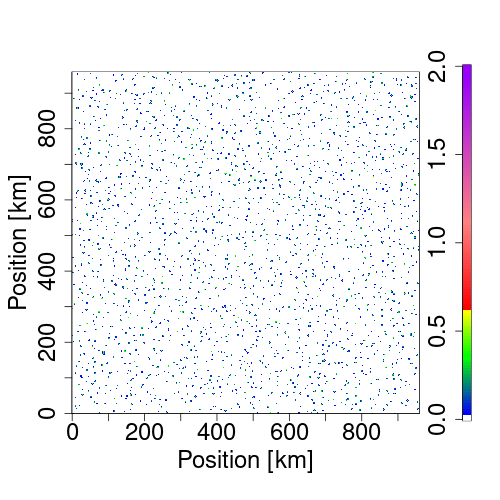
\includegraphics[height=0.35\linewidth,trim=0cm 2.75cm 2.6cm 0cm, clip]{var1_daymean_T0_300K_ampl_4_1km_large_1-96.png}}
\put(5,2){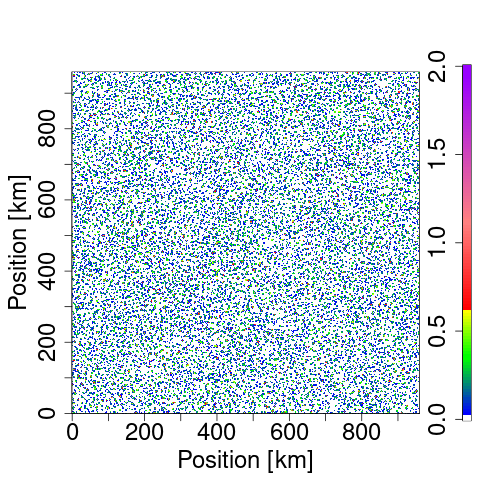
\includegraphics[trim={2.4cm 2.75cm 2.6cm 0cm}, clip, height=0.35\linewidth]{var1_daymean_T0_300K_ampl_4_1km_large_289-384.png}}
\put(60,2){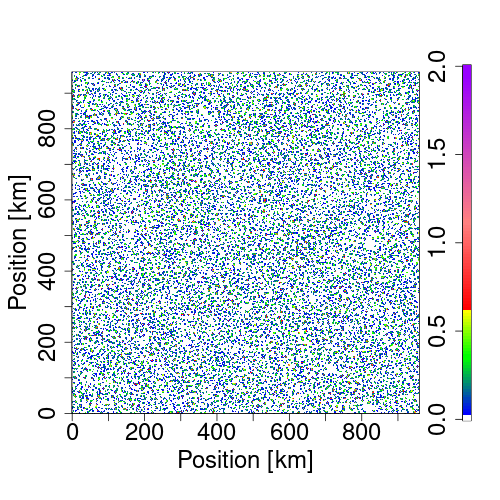
\includegraphics[trim={2.4cm 2.75cm 0cm 0cm}, clip, height=0.35\linewidth]{var1_daymean_T0_300K_ampl_4_1km_large_385-480.png}}
\put(-60,-65){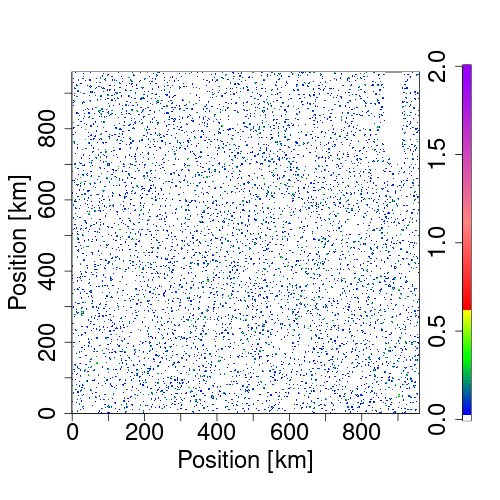
\includegraphics[trim={0cm 0cm 2.6cm 1.75cm}, clip, height=0.37\linewidth]{var1_daymean_T0_300K_ampl_10_1km_large_1-144.png}}
\put(5,-65){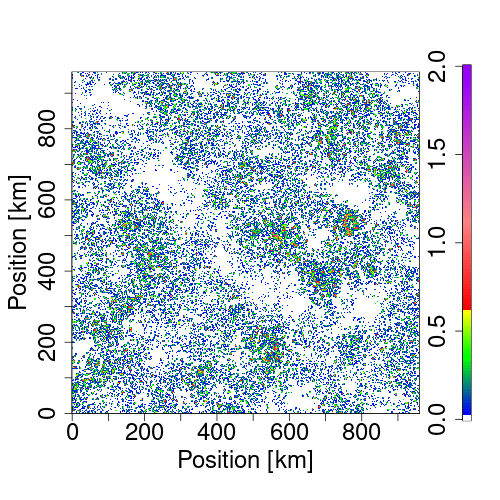
\includegraphics[trim={2.4cm 0cm 2.6cm 1.75cm}, clip, height=0.37\linewidth]{var1_daymean_T0_300K_ampl_10_1km_large_433-576.png}}
\put(60,-65){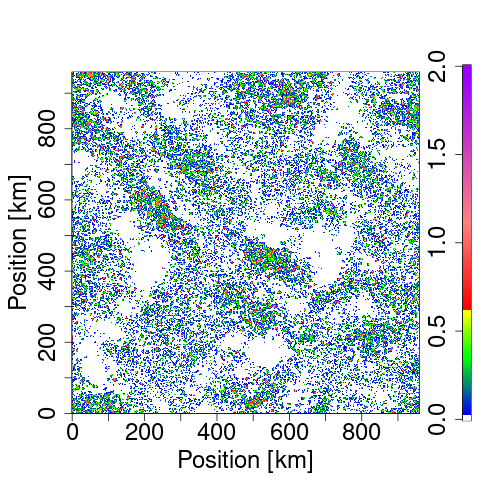
\includegraphics[trim={2.4cm 0cm 2.6cm 1.75cm}, clip, height=0.37\linewidth]{var1_daymean_T0_300K_ampl_10_1km_large_577-720.png}}

\put(-58,56){
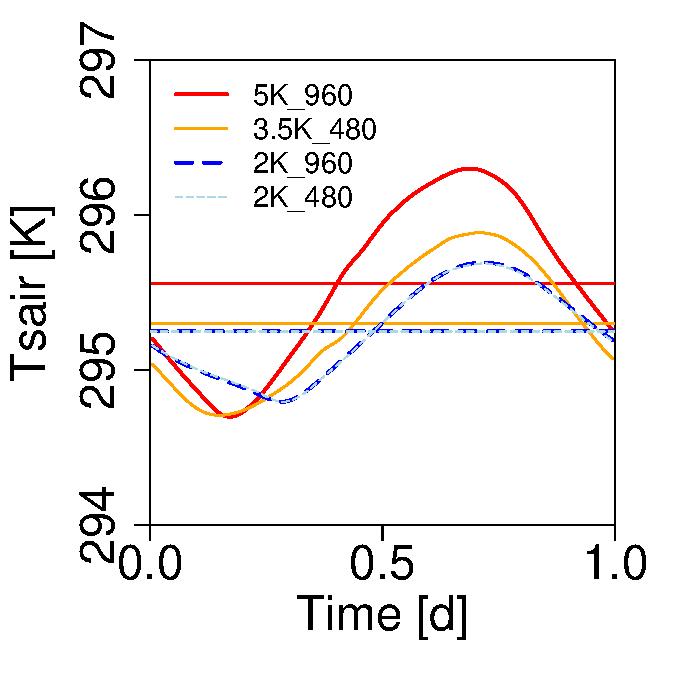
\includegraphics[trim={0 0 0cm 0}, clip, height=0.25\linewidth]{tsair_varying_ampl_timeseries_agg.pdf}}
\put(-15,56){
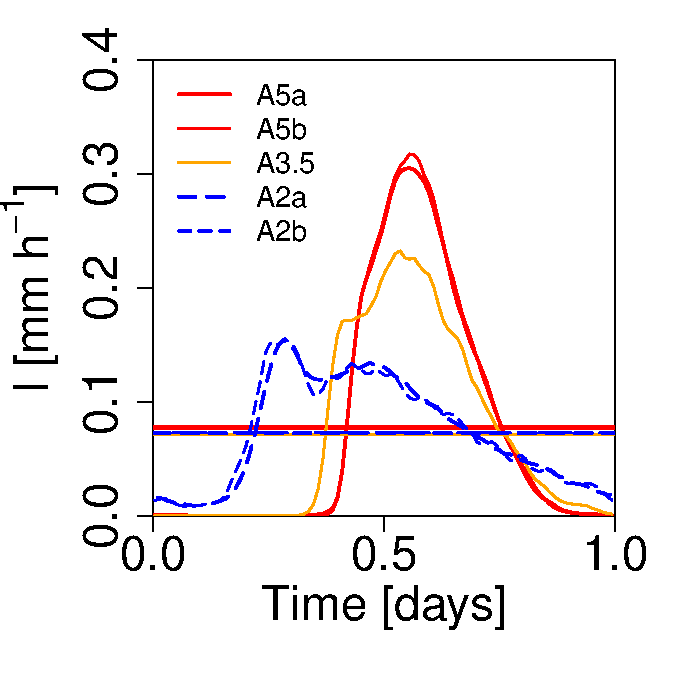
\includegraphics[trim={0 0 0cm 0}, clip, height=0.25\linewidth]{prcp_varying_ampl_timeseries_agg.pdf}}
\put(27,56){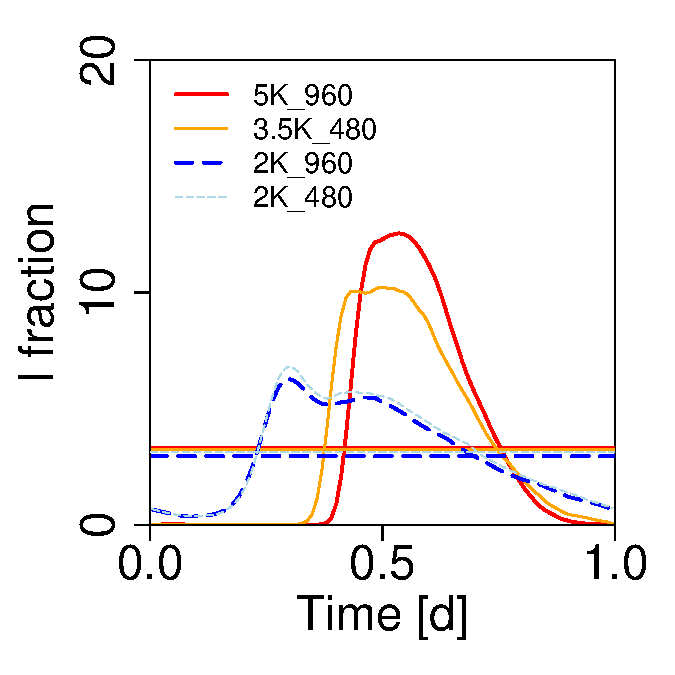
\includegraphics[trim={0 0 0cm 0}, clip, height=0.25\linewidth]{pfrac_varying_ampl_timeseries_agg.pdf}}
\put(70,56){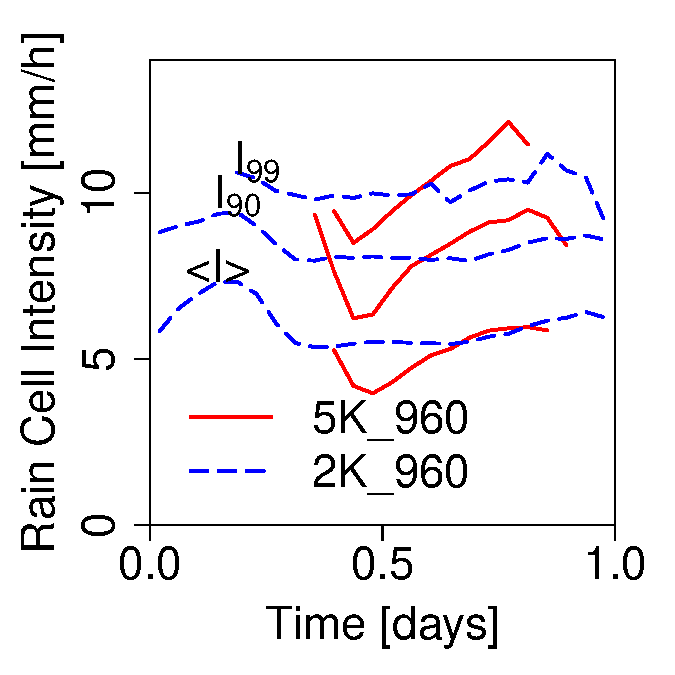
\includegraphics[trim={0 0 0cm 0}, clip, height=0.25\linewidth]{diurnal_heavy_precip.pdf}}

\put(-49,97){\large \bf a}
\put(-5,97){\large \bf b}
\put(35,97){\large \bf c}
\put(77,97){\large \bf d}

\put(-51,54){\large \bf e}
\put(4,54){\large \bf f}
\put(59,54){\large \bf g}
\put(-51,-2){\large \bf h}
\put(4,-2){\large \bf i}
\put(59,-2){\large \bf j}

\put(-50,47){\large $A2a$}
\put(-50,-10){\large $A5a$}

\put(10,37){\color{black}\line(0,-1){10}}
\put(10,27){\color{black}\line(1,0){10}}
\put(10,37){\color{black}\line(1,0){10}}
\put(20,37){\color{black}\line(0,-1){10}}

\put(10,-20){\color{black}\line(0,-1){10}}
\put(10,-30){\color{black}\line(1,0){10}}
\put(10,-20){\color{black}\line(1,0){10}}
\put(20,-20){\color{black}\line(0,-1){10}}

\put(65,37){\color{black}\line(0,-1){10}}
\put(65,27){\color{black}\line(1,0){10}}
\put(65,37){\color{black}\line(1,0){10}}
\put(75,37){\color{black}\line(0,-1){10}}

\put(65,-20){\color{black}\line(0,-1){10}}
\put(65,-30){\color{black}\line(1,0){10}}
\put(65,-20){\color{black}\line(1,0){10}}
\put(75,-20){\color{black}\line(0,-1){10}}

\end{overpic}
%\begin{picture}
%\put(0,15){\circle(20)}
%\end{picture}
\vspace{5cm}
\caption{{\bf Transition to a clustered rainfall state.}
{\bf a---d}, Diurnal cycles of domain averaged quantities.
%[here we might also want to show $T(6000m)$ and specific humidity.]
Each quantity was horizontally averaged. 
Time-series represents a compound diurnal cycle, where equal times of day were averaged over all available model days.
{\bf a}, Near-surface temperature for simulations with different imposed surface temperature amplitudes, as labeled in legend. 
Horizontal lines of corresponding colors represent the time average of each simulation.
{\bf b}, Analogous to (a), but for rain intensity.
{\bf c}, Analogous to (a), but for rain area fraction.
{\bf d}, Mean, 90'th and 99'th percentiles of rain intensity for $A5$ and $A2$, as labeled in the panel.
{\bf e}, Surface rainfall average during the first day ($t=1d$, spin up) for $A2$.
{\bf f}, Similar to (e), but for $t=3d$.
{\bf g}, Similar to (e), but for $t=4d$.
{\bf h---i}, Similar to (e)---(g), but for $A5$.
To highlight the spatial and temporal variation, boxes of side length $150\;km$ are shown at equal positions in panels f,g,i,j.
}
\label{fig:daily_mean}
\end{figure*}

\begin{figure}[ht]
\centering
\begin{overpic}[width=0.4\textwidth ]{dummy.pdf}
\put(-50,37){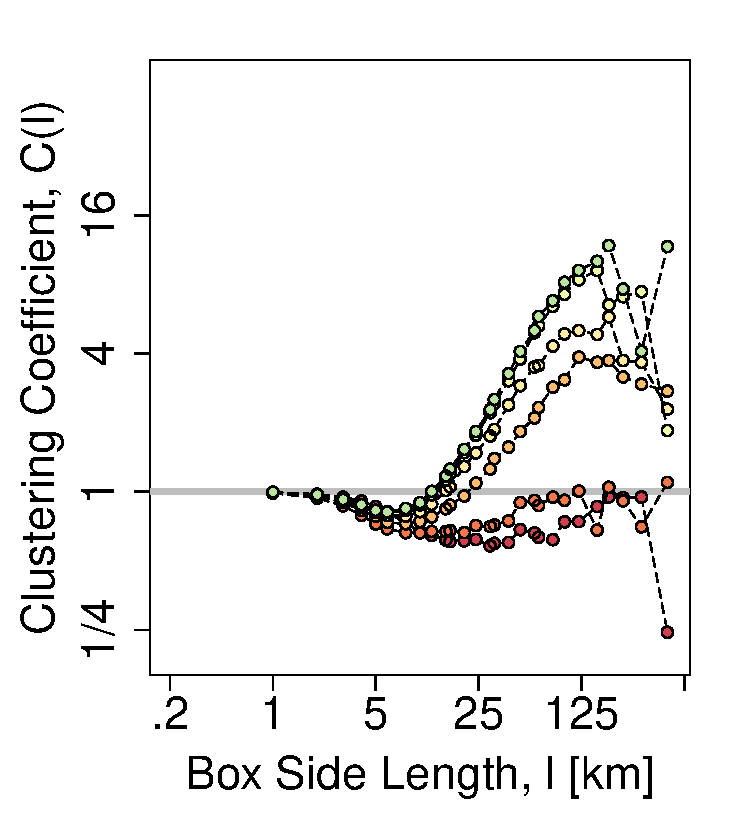
\includegraphics[trim={0cm 0cm 0cm 0cm}, clip, height=0.36\linewidth]{var_A5a.pdf}}
\put(5,37){\includegraphics[trim={0cm 0cm 0cm 0cm}, clip, height=0.36\linewidth]{{var_A3.5}.pdf}}
\put(60,37){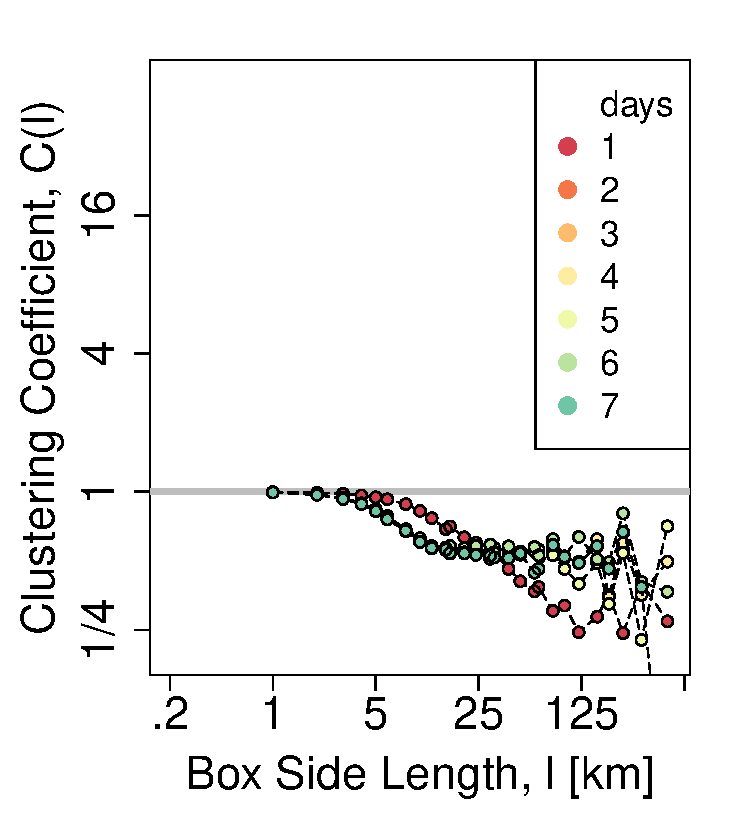
\includegraphics[trim={0cm 0cm 0cm 0cm}, clip, height=0.36\linewidth]{var_A2a.pdf}}
\put(-50,-25){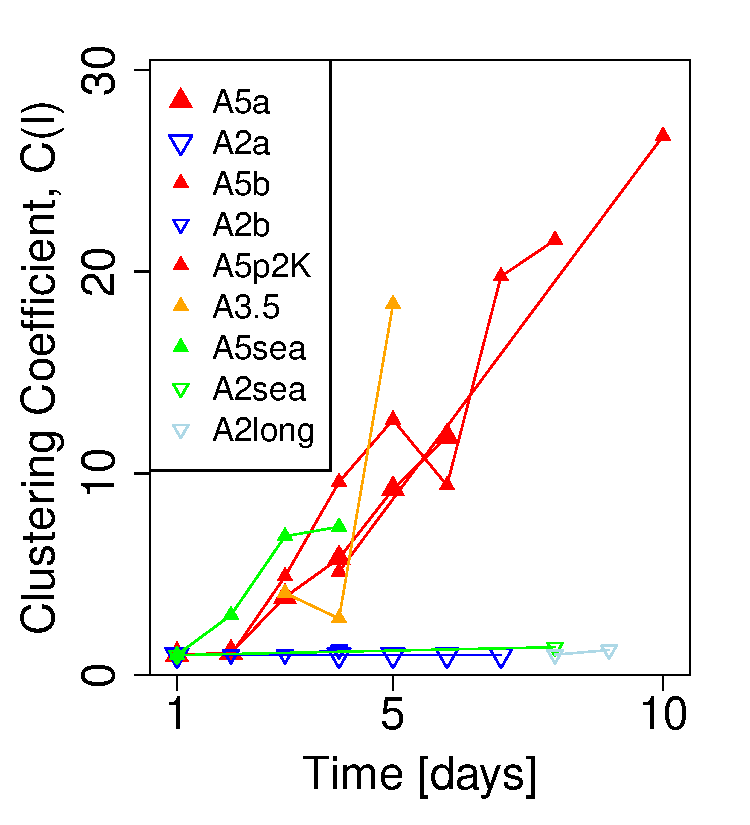
\includegraphics[trim={0cm 0cm 0cm 0cm}, clip, height=0.36\linewidth]{maxvar_vs_day.pdf}}
\put(5,-25){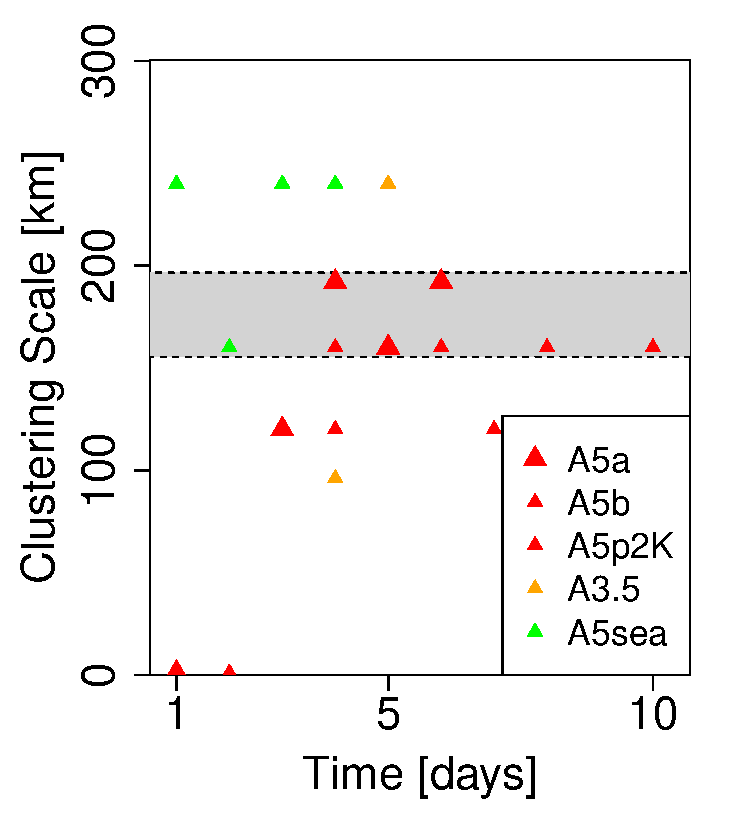
\includegraphics[trim={0cm 0cm 0cm 0cm}, clip, height=0.36\linewidth]{maxvarPos_vs_day.pdf}}
\put(60,-25){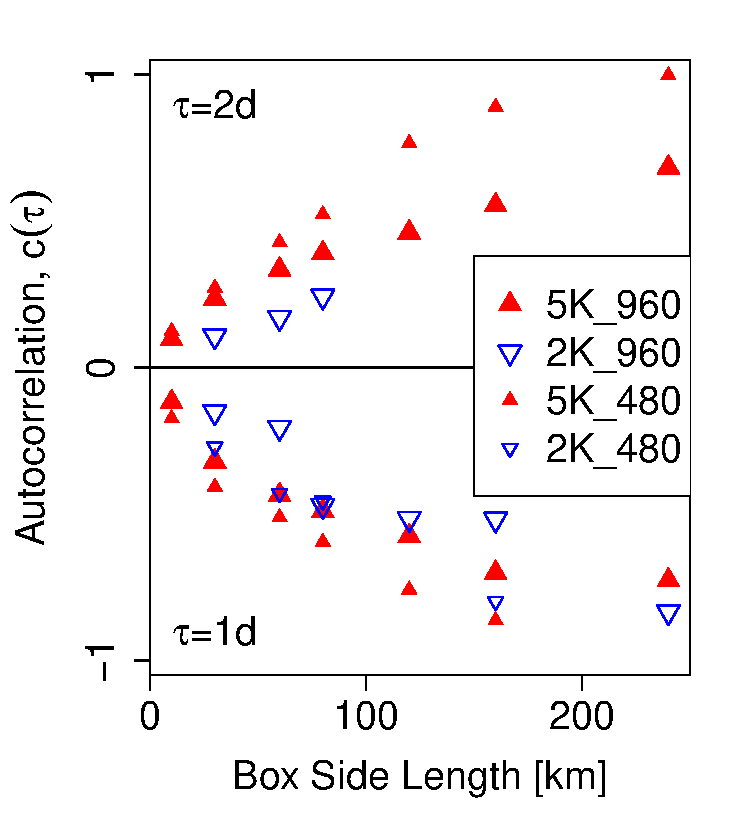
\includegraphics[trim={0cm 0cm 0cm 0cm}, clip, height=0.36\linewidth]{autocor_vs_day.pdf}}
\put(-40,97){\large \bf a}
\put(15,97){\large \bf b}
\put(70,97){\large \bf c}
\put(-40,35){\large \bf d}
\put(15,35){\large \bf e}
\put(70,35){\large \bf f}
\put(-38,90){ $A5a$}
\put( 17,90){ $A3.5$}
\put( 72,90){ $A2a$}

%\put(-33,25){\large $A5$, $A3.5$}
%\put( 12,){\large $A3.5$}
%\put(-18,-8){\large $A2$}

\put(-36,53){  regular}
\put(-36,75){  clustered}

\end{overpic}
\vspace{1.5cm}
\caption{{\bf Quantifying clustering using spatial variance.}
{\bf a}, Spatial variance at different box sizes for $A5$.
Curves of colors ranging from red (day one) to green (day six) correspond to increasing time.
Note that at small scales ($\sim 10\;km$) or early times ($t<2\;d$) rain events are distributed regularly, while at larger scales ($\sim 150\;km$) and later times, events are clustered.
Note the double-logarithmic axis scaling.
{\bf b}, Analogous to (a), but for $A3.5$.
{\bf c}, Analogous to (a), but for $A2$. 
Note that the normalized variance remains in the regular range and does not exceed unity.
{\bf d}, Peaks of variance anomalies vs. time for different simulations [mark them in legend]. 
Note the general increase for large $\Delta T$ but flat behavior for small $\Delta T$.
{\bf e}, Scales of clustering, i.e. the peak position in all clustered distributions $A3.5$ and $A5$. The gray shaded area marks the standard error of $l_{max}$, averaged over all times $t\geq 3d$. 
{\bf f}, Autocorrelation coefficient $c(\tau)$ for $\tau=1$ and $\tau=2$, showing increasing autocorrelation with scale for both A2 and A5.
}
\label{fig:quantifying_clustering}
\end{figure}

\begin{figure}[ht]
\centering
\begin{overpic}[width=0.4\textwidth]{dummy.pdf}

\put(-55,15){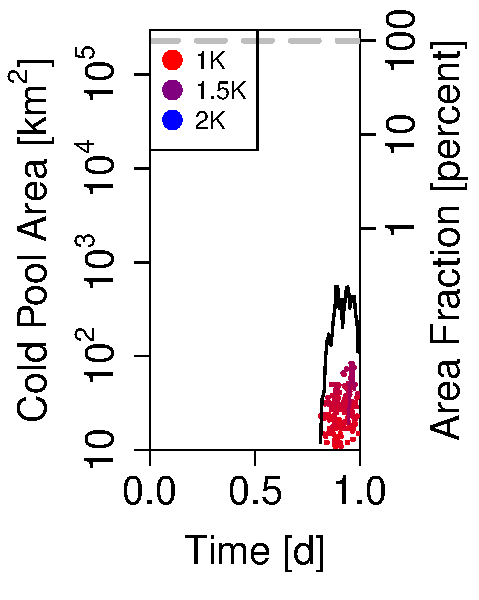
\includegraphics[trim={0cm 2.15cm 1.8cm 0cm}, clip, height=0.205\linewidth]{temp_depr_timeseries_area_A2b_day_1-288.pdf}}
\put(-28,15){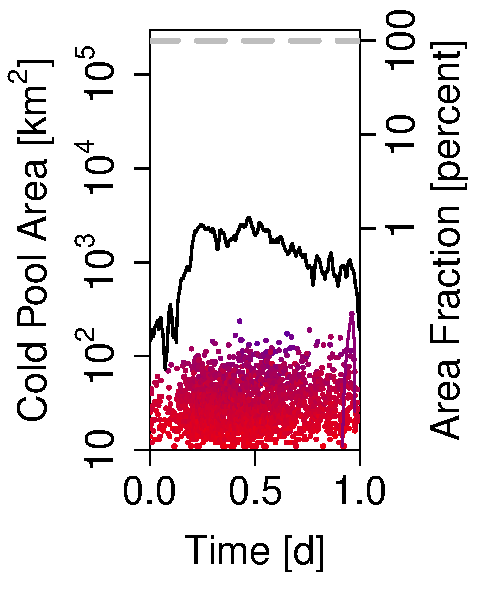
\includegraphics[trim={1.95cm 2.15cm 1.8cm 0cm}, clip, height=.205\linewidth]{temp_depr_timeseries_area_A2b_day_289-576.pdf}}
\put(-10,15){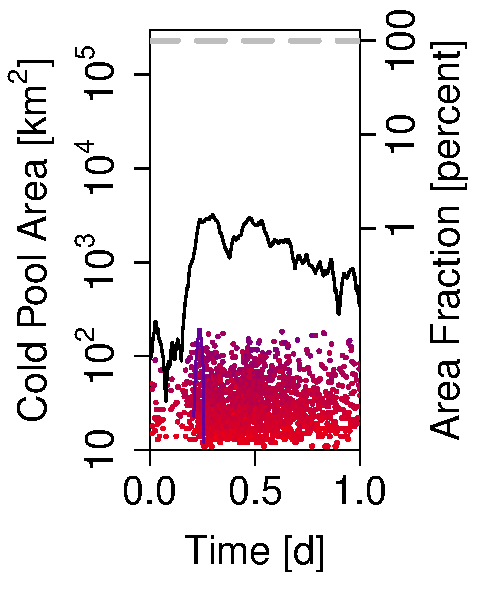
\includegraphics[trim={1.95cm 2.15cm 0cm 0cm}, clip, height=0.205\linewidth]{temp_depr_timeseries_area_A2b_day_865-1172.pdf}}

\put(-55,-31){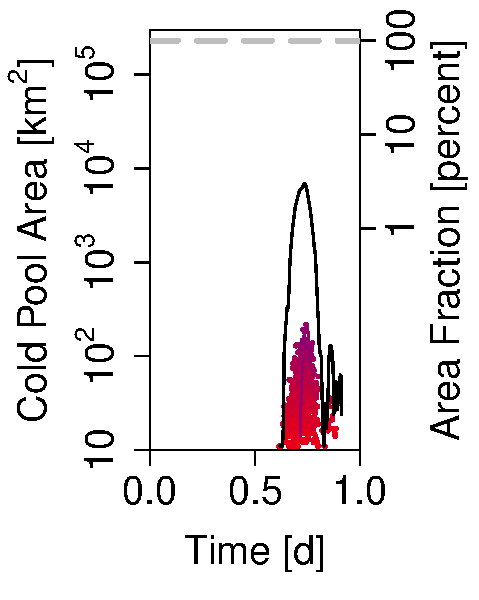
\includegraphics[trim={0cm 0cm 1.8cm 0cm}, clip, height=0.255\linewidth]{temp_depr_timeseries_area_A5b_day_1-288.pdf}}
\put(-28,-31){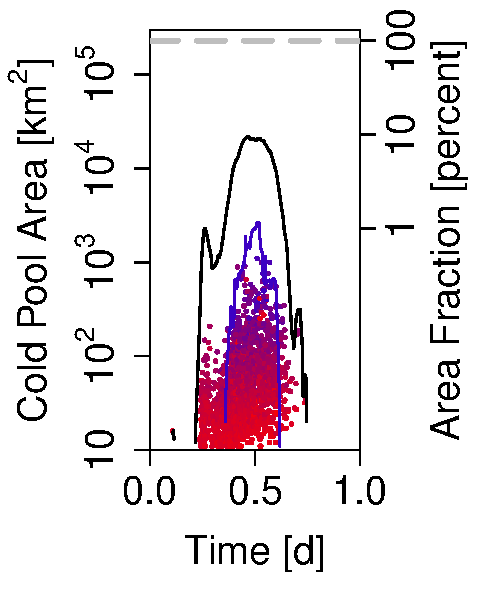
\includegraphics[trim={1.95cm 0cm 1.8cm 0cm}, clip, height=0.255\linewidth]{temp_depr_timeseries_area_A5b_day_333-600.pdf}}
\put(-10,-31){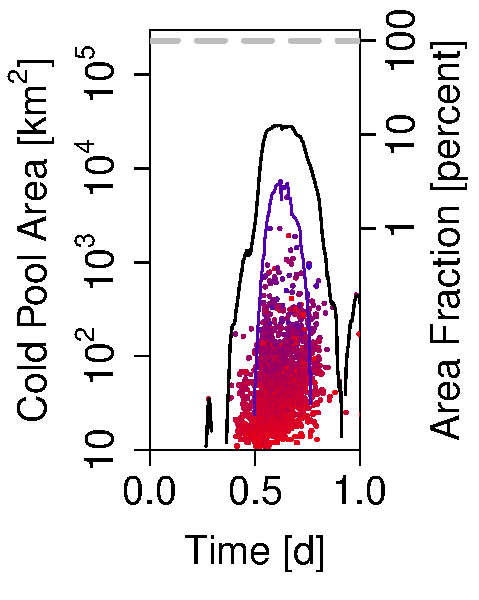
\includegraphics[trim={1.95cm 0cm 0cm 0cm}, clip, height=0.255\linewidth]{temp_depr_timeseries_area_A5b_day_909-1176.pdf}}

\put(13,16){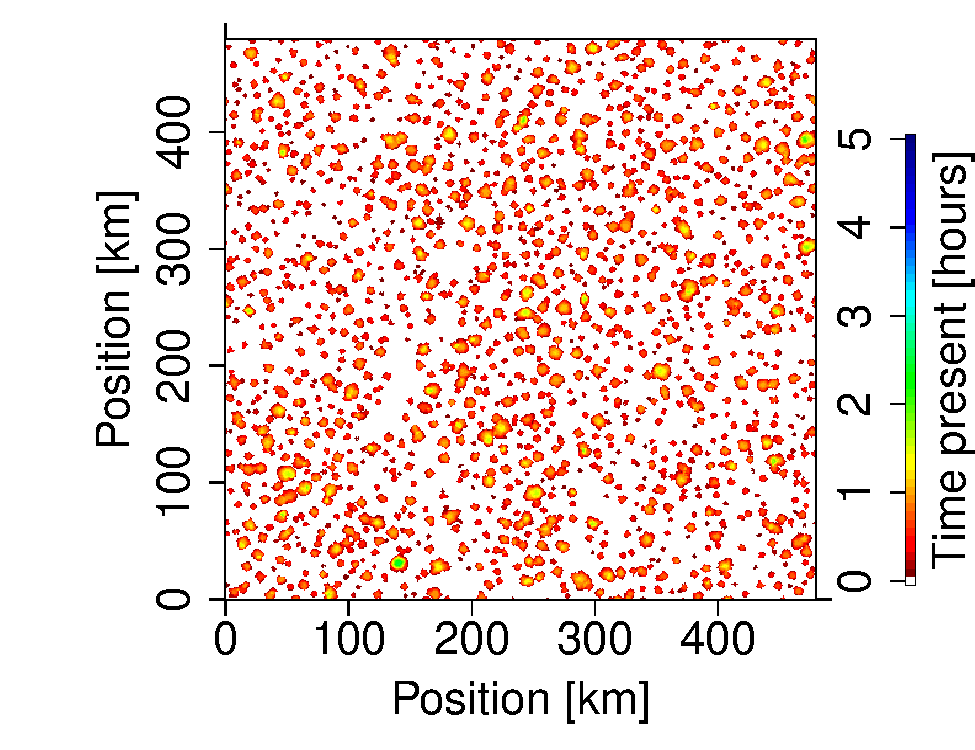
\includegraphics[trim={.0cm 2.25cm 0cm 0cm}, clip, height=0.20\linewidth]{cp_presence_T0_300K_ampl_4_1km_865-1172.pdf}}
\put(13,-28){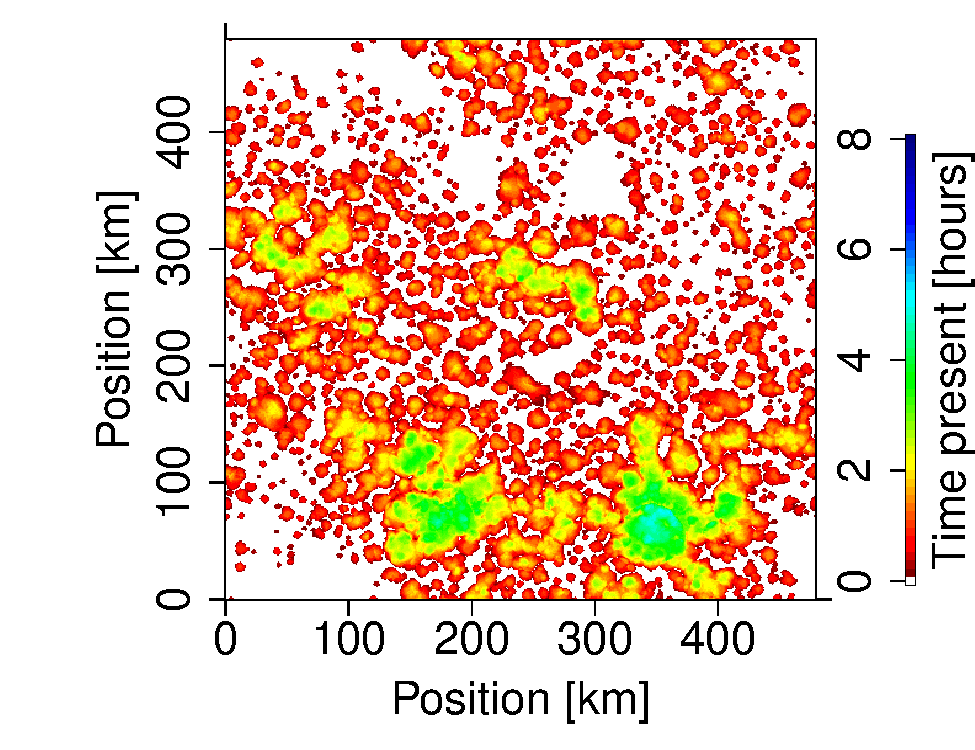
\includegraphics[trim={.0cm 0cm 0cm 0cm}, clip,height=0.24\linewidth]{cp_presence_T0_300K_ampl_10_1km_909-1176.pdf}}


\put(70,16){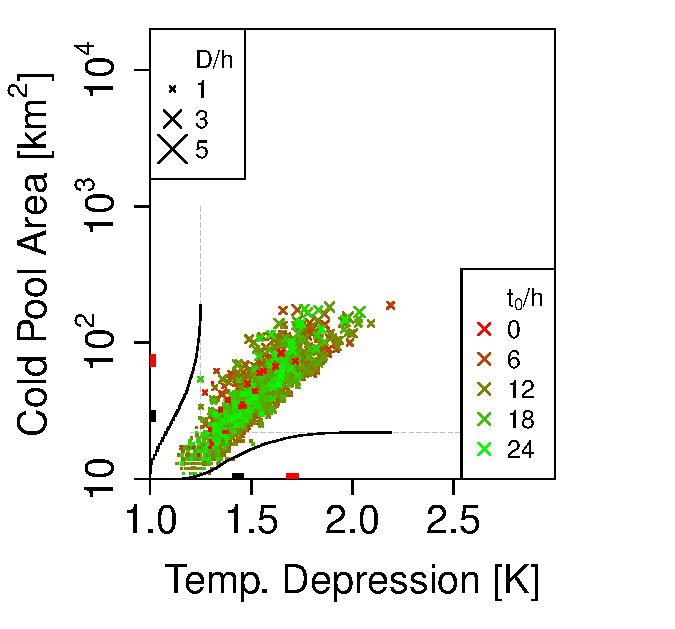
\includegraphics[trim={.0cm 2.15cm 0cm 0cm}, clip, width=0.27\linewidth]{temp_depr_scatterplot_area_A2b_day_865-1172.pdf}}
\put(70,-30){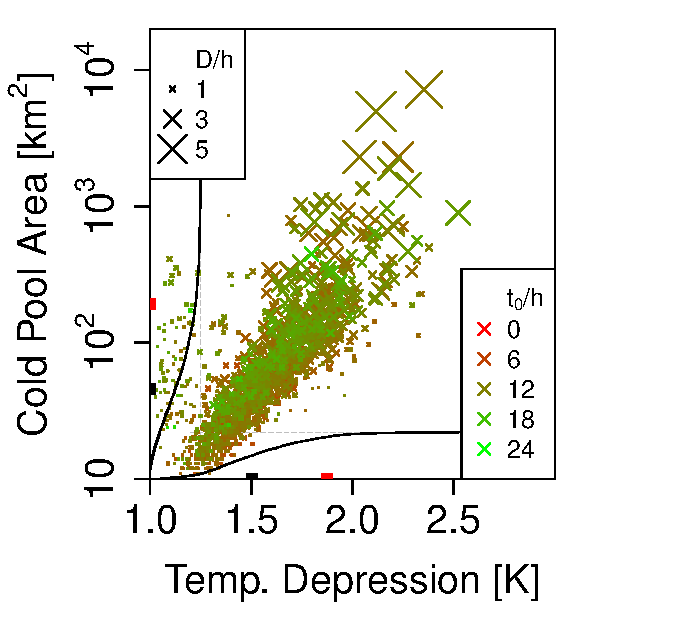
\includegraphics[trim={.0cm 0cm 0cm 0cm}, clip,width=0.27\linewidth]{temp_depr_scatterplot_area_A5b_day_909-1176.pdf}}

%\put(70,7){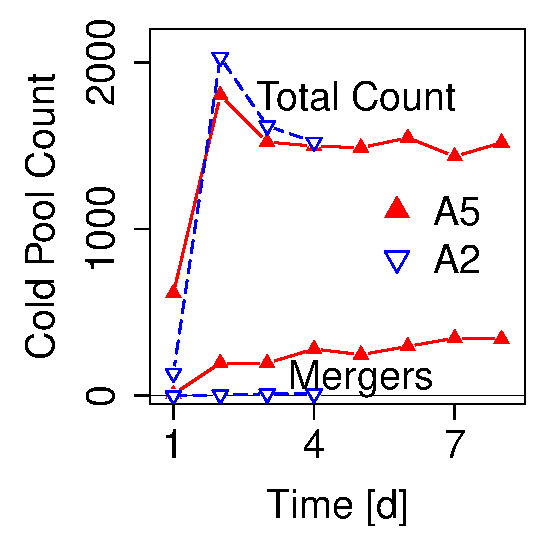
\includegraphics[trim={.0cm 0cm 0cm 0cm}, clip,height=0.23\linewidth]{merge_split_stats.pdf}}

\put(-43,50){\bf a}
\put(-26,50){\bf b}
\put(-7,50){\bf c}
\put(26,50){\bf d}

\put(-43,12){\bf e}
\put(-26,12){\bf f}
\put(-7,12){\bf g}
\put(26,12){\bf h}

%\put(-45,72){\large $\Delta T=5\;K$}
%\put(-45,25){\large $\Delta T=2\;K$}
\end{overpic}
\vspace{2cm}
\caption{{\bf Cold pool merging and deepening.}
{\bf a}, Occurrence time, maximum area, and average temperature depression (colors from red to blue) of CPs on day one of the A2 simulation. The black curve indicates the total CP area at each time.
{\bf b,c}, Analogous to (a), but for days two and three of A2.
{\bf d}, Areas covered by CPs during day three of A2, color shading indicates the duration during which CPs were present.
{\bf e---h}, Analogous to (a)---(d), but for A5.
Note the logarithmic vertical axis scale in (a)---(c) and (e)---(g).
}
\label{fig:CP_merging}
\end{figure}

\begin{figure}[ht]
\centering
\begin{overpic}[width=0.4\textwidth ]{dummy.pdf}
\put(-35,71){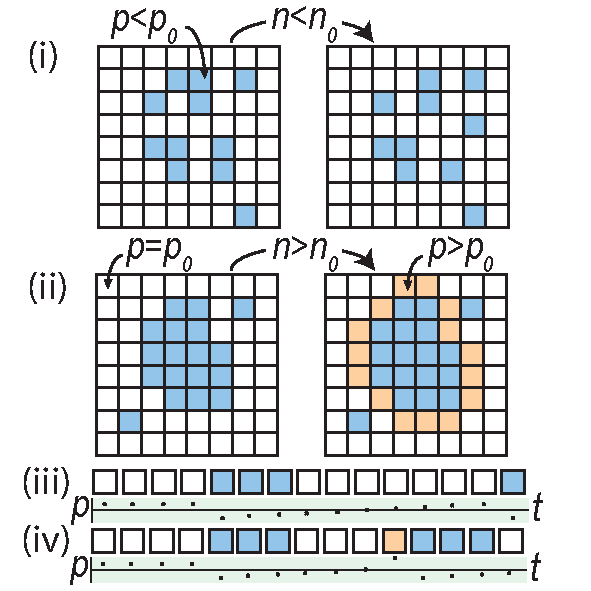
\includegraphics[trim={0cm 0cm 0cm 0cm}, clip, height=0.33\linewidth]{schematic_simplified_supercell.pdf}}
\put(22,100){\includegraphics[trim={.0cm 0cm 0cm 0cm}, clip,height=0.17\linewidth]{{variance_checkerboard_q=0.100000}.pdf}}
\put(23,85){\includegraphics[trim={2cm 2cm 4cm 0cm}, clip,height=0.08\linewidth]{{checkerboard_simple_p0=2_N=10_ts=0.dat}.png}}
\put(35,85){\includegraphics[trim={2cm 2cm 4cm 0cm}, clip,height=0.08\linewidth]{{checkerboard_simple_p0=2_N=10_ts=1.dat}.png}}
\put(47,85){\includegraphics[trim={2cm 2cm 4cm 0cm}, clip,height=0.08\linewidth]{{checkerboard_simple_p0=2_N=10_ts=2.dat}.png}}
\put(59,85){\includegraphics[trim={2cm 2cm 4cm 0cm}, clip,height=0.08\linewidth]{{checkerboard_simple_p0=2_N=10_ts=3.dat}.png}}
\put(23,71){\includegraphics[trim={2cm 2cm 4cm 0cm}, clip,height=0.08\linewidth]{{checkerboard_simple_p0=1_N=10_ts=0.dat}.png}}
\put(35,71){\includegraphics[trim={2cm 2cm 4cm 0cm}, clip,height=0.08\linewidth]{{checkerboard_simple_p0=1_N=10_ts=1.dat}.png}}
\put(47,71){\includegraphics[trim={2cm 2cm 4cm 0cm}, clip,height=0.08\linewidth]{{checkerboard_simple_p0=1_N=10_ts=2.dat}.png}}
\put(59,71){\includegraphics[trim={2cm 2cm 4cm 0cm}, clip,height=0.08\linewidth]{{checkerboard_simple_p0=1_N=10_ts=3.dat}.png}}
\put(-40,-3){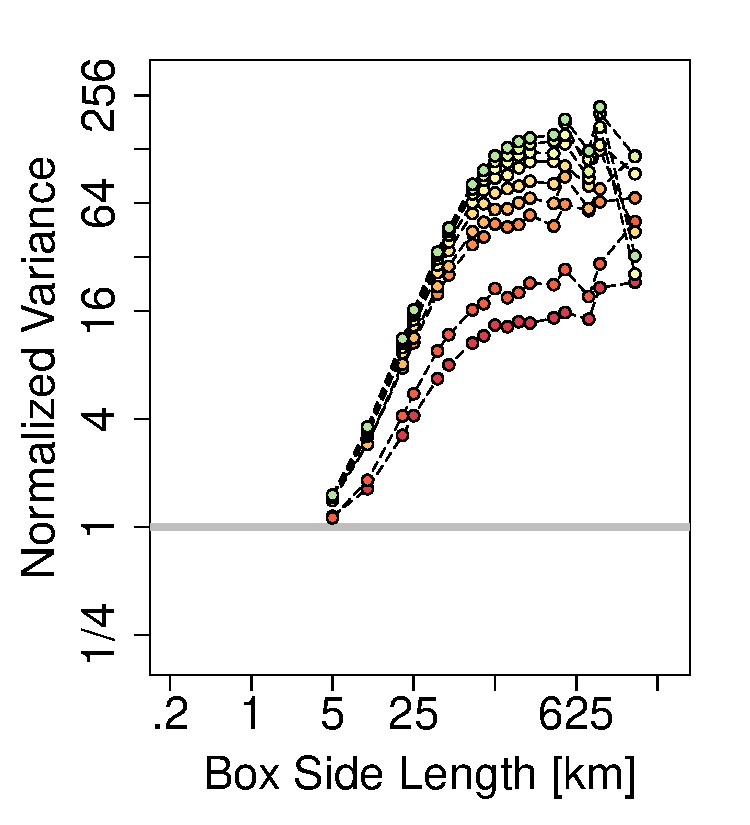
\includegraphics[trim={0cm 0cm 0cm 0cm}, clip, height=0.4\linewidth]{var_Ta5.pdf}}
\put(20,-3){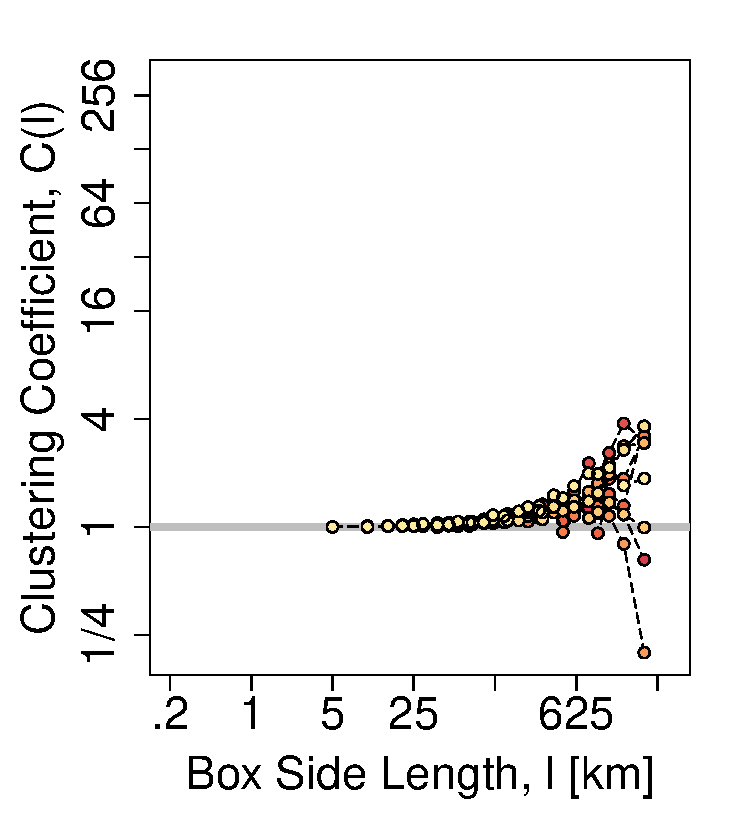
\includegraphics[trim={2cm 0cm 0cm 0cm}, clip, height=0.4\linewidth]{var_Ta1.pdf}}
\put(22,23){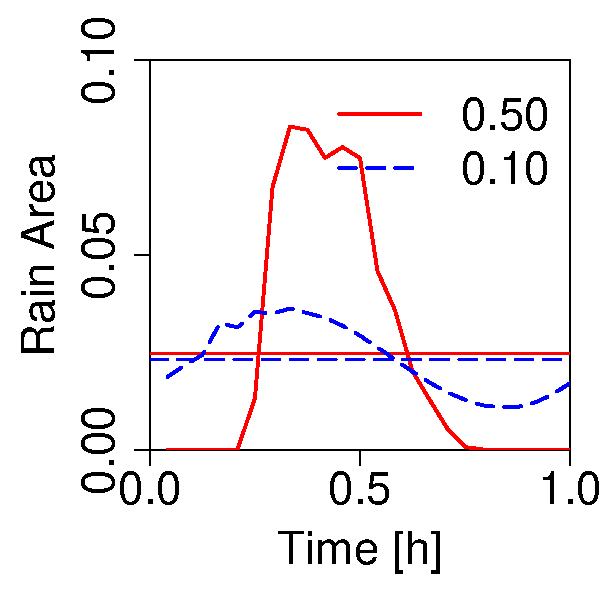
\includegraphics[trim={0cm 0cm 0cm 0cm}, clip, height=0.23\linewidth]{simple_model_rainarea_composite.pdf}}

\put(-35,126){\large \bf a}
\put(18,126){\large \bf b}
\put(-35,65){\large \bf c}
\put(18,65){\large \bf d}

\put(23,97){day 1}
\put(35,97){2}
\put(47,97){3}
\put(59,97){4}

\put(-27,15){\large large $T_a$}
\put( 22,15){\large small $T_a$}
%\put( 62,100){\large $\Delta T=2\;K$}
\end{overpic}
\vspace{0cm}
\caption{{\bf A simplified model explains the clustering.}
{\bf a}, Schematic for the simplified model dynamics.
(i) Low-density domain with vacant (white, probability $p_0$) and active (blue, probability $p<p_0$) sites;
(ii) Similar to (i) but for high density, showing also boundary sites (orange) with increased probability $p>p_0$.
(iii) Possible time series for a single site in (ii).
The green shaded area indicates a possible time series of $p$.
(iv) Similar to (iii) but corresponding to (ii). 
{\bf b}, Simple checkerboard model, explaining the increase in variance over time for large $T_a$ (red symbols) and small $T_a$ (blue symbols).
The grids below show the patterns at days 1---4 for large and small $T_a$, respectively.
Note the increasing anti-correlations for large $T_a$.
{\bf c}, Spatial variance at different box sizes for a large value of $T_a$, 
analogous to Fig.~\ref{fig:quantifying_clustering} but for the simplified model.
Curves of colors ranging from red to green correspond to increasing days.
For larger scales and later times, events are clustered.
Note the double-logarithmic axis scaling.
{\bf d}, Analogous to (c), but for small $T_a$.
}
\label{fig:quantifying_clustering_simplified}
\end{figure}

\section*{Discussion}\label{sec:discussions}
Our study analyses the spontaneous emergence of convective clustering, when the amplitude of the diurnal cycle is varied. 
During mid-latitude summer, extreme rainfall events and flash floods have been found to occur more frequently during long periods of pronounced heating \cite{coumou2012decade}.
The findings here suggest, that the clustering, and thereby the potential for flash floods, increases from day to day, and reaches the largest potential at the scale of $l_{max}\approx 150\;km$.
We have also addressed clustering over a sea surface, finding analogous results:
not the mean, but the amplitude of surface temperature gives rise to clustering.
Increasing model horizontal resolution to $.5$ or $.2$ $km$ (Fig.~\ref{fig:daily_sum_higher_res}) leads to even stronger clustering effects, in agreement with recent findings with a realistic continental topography \cite{rasp2018variability}.

In convective self-aggregation, the common explanation for clustering invokes arguments based on circulation changes.
Remarkably, the memory enabling clustering in the present work is purely thermodynamically-driven, we do not detect any sustained changes of circulation that harbor a memory from one day to the next.
The findings hence suggest two possible "shortcuts" to self-aggregation over the ocean: 
(i) at times, sea surface temperature oscillations may be sufficient in kick-starting a clustering;
(ii) clustering may emerge over land surfaces and is then advected over the sea.
Both explanations require that clustering can be sustainable once formed --- a requirement consistent with hysteresis effects suggested earlier \cite{muller2015favors}.
In our simplified models, hysteresis is, in fact, easy to achieve: once an imbalance between neighboring grid cells is reached, sustained redistributions will be possible, even when the overall event number density is then lowered.

The present work can be seen as interpolating between the paradigmatic RCE setup for oceanic convection and typical boundary conditions for continental convection. 
The findings raise questions on the production of extreme downpours over land and their intensification over time, as well as the origin of clustering over ocean.
Future research should probe, whether a state of self-aggregation can be reached more quickly when sea-surface temperatures transiently oscillate --- thereby exciting initial clustering on the scale of $l_{max}$.

\newpage
\clearpage
\section*{Materials and Methods}\label{sec:methods}
\noindent
{\bf Large-eddy model, boundary and initial conditions.}
We simulate the convective atmosphere using the University of California, Los Angeles (UCLA) Large Eddy Simulation (LES) model with sub-grid scale turbulence parametrized after Smagorinsky \cite{smagorinsky1963general}, a delta four-stream radiation scheme \cite{pincus2009monte} and a two-moment cloud microphysics scheme \cite{stevens2005evaluation}. 
Rain evaporation is implemented after \citeauthor{seifert2006two}, \citeyear{seifert2006two}.
Diurnally oscillating, spatially homogeneous, surface temperature ($T_s(t)$) boundary conditions are prescribed, with
\begin{eqnarray}
    T_s(t)=\overline{T_{s}}-T_{a} \cos{(2\pi\;t/t_0)}\;,
\end{eqnarray}
\noindent
with $\overline{T_{s}}=298\;K$, $t_0=24\;h$ is the duration of the simulated model day, and the overline representing the temporal average.
Surface fluxes are computed interactively and depend on the vertical temperature and humidity gradients as well as horizontal wind speed, which is approximated using Monin-Obukhov similarity theory.
Temperature and humidity were initialized using observed profiles that represent potentially convective conditions.
%data from observed summertime mid-latitude conditions where convection had occurred in order to establish an initially unstable atmosphere. 
However, due to the repeated diurnal cycle forcing, the system eventually establishes a self-consistent vertical temperature and moisture profile.

\noindent
{\bf Model grid, dynamics, and output.}
The model numerically integrates the anelastic equations of motion on a regular horizontal domain with varying horizontal grid spacing $dx$ and periodic boundary conditions (Tab. \ref{tab:experiments}). 
Vertical model resolution is $100\;,m$ below $1\;km$, stretches to $200\;m$ near $6\;km$ and reaching $400\;m$ in the upper layers, with the model top located at $16.5\;km$.
Horizontal resolution $dx$ and domain size vary (Tab.~\ref{tab:experiments}). 
The Coriolis force and the mean wind were set to zero with weak random initial perturbations added as noise to break complete spatial symmetry. 
No large scale forcing was imposed, ensuring that the only driving force for convection was buoyancy and the forced lifting through cold pool interaction.
For all two and three-dimensional model variables, the output time step varies between experiments between $\Delta t_{out}=5\;min$ and $15\;min$. 
At each output time step (Tab.~\ref{tab:experiments}), instantaneous surface precipitation intensity, as well as the three-dimensional moisture and velocity fields, are recorded for the entire model domain. 
Additionally, at 30-second and five-minute intervals, respectively, spatially-averaged as well as horizontally averaged time-series were extracted from the numerical experiments.

\noindent
{\bf Sensitivity experiments.} 
The principal focus of this study is the response to different values of surface temperature amplitude, $T_a$. 
The main experiments (A5a, A2a, A5b, A2b) were carried out at $T_s=298\;K$, contrasted $T_a=2\;K$ and $T_a=5\;K$ (Tab.~\ref{tab:experiments}) and used $dx=1\;km$ horizontal model resolution.
One intermediate value of $T_a=3.5\;K$ was tested to further constraint the transition to clustering.
These simulations assumed, that surface latent heat fluxes occurred at $70$ percent of their potential value --- mimicking a land surface, which is reasonable given the mean surface latent and sensible heat fluxes of $LHF\approx 57\;W/m^2$ and $SHF\approx 18\;W/m^2$, yielding a Bowen ratio of $B\approx .30$, realistic for forested land. 
These main experiments already explore domain size effects, as the clustering observed could be influenced by the finite system size --- yielding a good degree of consistency.
To test for sensitivity to a range of further modifications, experiments were conducted to explore: lateral model resolution (A5c, A5d), where $dx=.5\;km$ and $dx=.2\;km$ were used; cold pool strength (A5vent05, A5vent001), where the ventilation coefficients $a_v$ and $b_v$ in Eq. 24 of \citeauthor{seifert2006two} \citeyear{seifert2006two} were reduced to $.5$ and $.01$ of their default values; and surface conditions, where surface evaporation was raised to its potential value, mimicking a sea surface ($B\approx .15$, {\it Details}: Tab.~\ref{tab:experiments}).
%All domains used had square horizontal geometry of $L\times L$, where the linear domain size $L$ took the values $240$, $480$ and $960$ $km$.
%Lateral resolution $dx$ took the values $.2$, $.5$ and $1.0$ $km$.
%Cold pool strength is dependent on the amount of rain evaporation. To vary cold pool strength, the value of the ventilation coefficient was modified from its default value \cite{seifert2006two} by diminishing this by a factor $.5$ and $.01$ --- resulting in substantially smaller temperature anomalies below precipitating clouds and weaker cold pools.
%Surface evaporation was modified by using a sea surface, hence potential evaporation, and one where potential evaporation was reduced to 70 percent ({\it compare:} \citeauthor{moseley2016intensification}, \citeyear{moseley2016intensification}).

\noindent
{\bf Rain cell and cold pool tracking.}
In all experiments, rain cells were tracked by the Iterative Rain Cell Tracking Method (IRT, \cite{moseley2019statistical}).
In the two-dimensional surface precipitation field corresponding to any output timeframe, the IRT first detects all spatially contiguous patches of rain intensities exceeding a threshold $I_0=.5\;mm\;h^{-1}$, termed {\it rain objects}.
Tracks and then identified, by determining and rain objects that overlap from one output timestep to the next. 
The threshold value $\theta$ was set to unity, meaning that, the case of merging, the track of larger area is continued under the same track ID.
In our variance analysis, we use the set of coordinates formed by the initial position of each track, which is defined here as the precipitation-weighted center of mass of the initial rain objects belonging to each track.
The positions of all subsequent rain objects of the same track are discarded in our variance analysis, to avoid artifacts from double counting of the positions of the nearly collocated objects.

To account for possible changes in the cold pool extent between the different simulations, cold pools were tracked by a simple temperature depression method.
In this method, the IRT was modified, such that at any timestep any grid box with a temperature depression exceeding a threshold of one Kelvin was recorded.
As for rainfall, spatially contiguous patches of temperature depression were collected into objects and assigned indexes.
To increase the signal, only objects exceeding an area threshold of ten $\;km^2$ were considered.
Stepping forward in time, overlapping objects were identified and considered to be the same cold pool track.
The threshold ratio $\theta$ was again set to unity \cite{moseley2019statistical}.

\noindent
{\bf Simplified supercell model.}
A square lattice of $L\times L$ sites is initialized, where the area of each site is taken as the average area $a_0$ occupied by a single convective rain cell, $a_0\approx 4km\times 4km$. 
The total domain area $A$ hence is $A\equiv a_0L^2$.
Our model builds on the assumption, that boundary layer processes are local and fast, whereas the free troposphere acts as a "bath" of large heat capacity, where heat is quickly redistributed through gravity waves \cite{bretherton1989gravity}. 
The model incorporates three fundamental processes affecting event initiation: 
(1) spontaneous initiation due to the moderate drive of the diurnal cycle temperature forcing;
(2) refractory dynamics due to cold pools; 
(3) strong activation ahead of cold pool fronts.
Below we discuss the estimation of model parameters for these processes.
%All three processes are taken to occur, when the convective inhibition (CIN) is overcome.

\noindent
{\it Spontaneous activation.}
To define a vertical temperature gradient, we consider quantities $T_{bl}$ and $T_{ft}$, which represent the deviation of the boundary layer and free-tropospheric temperature from their assumed steady-state values.
$T_{bl}(t)$ is prescribed and oscillates harmonically as $T_{bl}(t)=-t_a \cos (2\pi t/t_0)$, where $t_0=1\;d$.
Free-troposphere temperature $T_{ft}$ is initialized to zero.
We also define the temperature difference $\Delta T\equiv T_{bl}-T_{ft}$ and its normalized version $\Delta T'\equiv \Delta T/\Delta T_0$, where the reference scale $\Delta T_0\approx .3\;K$ is taken as two standard deviations of simulated near-surface temperature.
$\Delta T'$ serves as a proxy for both convective available potential energy (CAPE) and convective inhibition (CIN).
The basic dynamics proceeds in discrete model timesteps of $.5$ $h$, reflecting the typical timescale of convective cloud formation. 
At each timestep, the default probability $p_0$ for a vacant site to become active is taken as
\begin{equation}
    p_0=\begin{cases}
    0 & \text{if $\Delta T'<0$}\\
    \Delta T' & \text{if $0<\Delta T'<1$}\\
    1 & \text{if $\Delta T'>1$}\;.
    \end{cases}
    \label{eq:cases}
\end{equation}
Eq.~\ref{eq:cases} makes the qualitative assumption, that there is no activity at all for stratified conditions ($\Delta T'<0$) and events occur with certainty when the temperature gradient is much larger than typical fluctuations. 
Both of these limits could be softened, as could the assumption of linearity at intermediate $\Delta T'$, that is, one could equally argue for a smooth function of $\Delta T'$, such as an error function. 
Nonetheless, Eq.~\ref{eq:cases} captures the observed fact that more initial activity occurs when surface temperature changes quickly.
Without any further perturbations, the initiation probability $p_{ij}$ at each site $(i,j)$ will be equal, $p_{ij}=p_0$.

\noindent
{\it Spatial structure.} 
Notably, Eq.~\ref{eq:cases} does not depend on the position within the lattice. 
Spatial structure is caused by local modifications ({\it compare}: Fig.~\ref{fig:quantifying_clustering_simplified}a).
Cold pools have two effects: reduction of local temperature and reduction of local humidity. 
However, the recovery timescale for the former is fast ($\tau_{cp}\approx 3\;h$), whereas that of the latter is slower ($\tau_{rec}\approx 1\;d$).
Temperature reduction dominates the density change and thereby the mechanical cold pool properties, whereas the latter crucially impacts on the local initiation probability.
To consider both, we take active sites to persist for $\tau_{cp}$, during which time no further activation is possible.
Simultaneously, the local probability $p_{ij}$ is reduced as $p_{ij}=p_0-p_{ref}\exp(-\delta t/\tau_{rec})$, where $\delta t$ is the time after the occurrence of the rain event and $p_{ref}>0$. 
$p_{ref}$ essentially controls the fidelity of the anti-correlation from day to day, and results are not qualitatively affected by it.

A supercell can occur, when an active cluster exceeds the threshold area $A_{crit}$ (Fig.~\ref{fig:quantifying_clustering_simplified}). 
While this is the case, and $\Delta T'>0$, the probability $p$ at each of the surrounding sites $(i,j)$ becomes $p_{ij}\rightarrow p_{ij}+p_{act}$, which acts to lower the barrier presented by CIN.
When $p_{ij}$ is no longer a surrounding site, the term $p_{act}$ is no longer applied.
The initiation probability $p_{ij}$ is then defined analogous to the one in Eq.~\ref{eq:cases}.

\noindent
{\it Radiative constraint.}
Generally, as $T_{bl}$ rises during the day as the surface is heated by insolation. 
$p_{ij}$ will then eventually become positive at some sites and rain cells can be produced there.
When this occurs, latent heat is transferred to the free troposphere, increasing $T_{ft}$, thus subsequently lowering $\Delta T$ and thereby $p_{ij}$.
Simultaneously, the site $(i,j)$ is shut down by the negative buoyancy effects through cold pool formation.
%Each occupied site will persist for $\tau_{cp}$, reflecting the relaxation time of temperature anomaly during a cold pool event and will then recover to an unoccupied site.
%The probability $p$ will relax to its equilibrium value at the relaxation rate $t_{rec}$.
The free tropospheric temperature will relax by heat loss ($P_{out}\approx 200\;W\;m^{-2}$) through outgoing thermal radiation. 
According to the Stefan-Boltzmann law, $P_{out}=\sigma T_{eff}^4$, with $\sigma\approx 5.7\times 10^{-8}W\;m^{-2}\;K^{-4}$ the Stefan-Boltzmann constant --- translating to an effective emission temperature $T_{eff}\approx 250\;K$. 
Through $P_{out}$, the free troposphere would hence cool by approximately $2\;K\;d^{-1}$.
As a crude estimate of the change in $T_{ft}$ through latent heat transfer, we estimate the free-tropospheric heat capacity $C_{ft}=M_{ft}c_{pd}$, assuming dry air.
$c_{pd}\approx 1\;kJ/kg$ and the mass of the free troposphere $M_{ft}=\int_{z=z_{LCL}}^{z_{top}}dz\;\rho(z)\approx 8\times 10^3\;kg$, using $z_{LCL}\approx 1\;km$ and $z_{top}\approx 16\;km$ for the lifting condensation level (LCL) and top of the troposphere, respectively.
Hence, $C_{ft}\approx 8\times 10^6\;Jm^{-2}K^{-1}$.
From rain cell tracking of our LES simulations, we obtain the average rain cell lifetime to be $\approx 1\;h$ (Tab.~\ref{tab:basic_stats}), the average cell area $a_0\approx 20\;km^2$ and the average cell rain rate of $\approx 4\;mm\;h^{-1}$ (Tab.~\ref{tab:basic_stats}), hence, each rain cell can be assumed to yield $M_{event}=4\;kg\;m^{-2}$ of liquid water.
Assuming that the corresponding latent heat was previously deposited in the free troposphere upon ascent, each rain event heats the free troposphere by $Q_{event}=L_v\;M_{event}$.
We take this heat to increase $T_{eff}$ accordingly by $\delta\;T_{eff}=Q_{event}/C_{ft}L^{2}$, where $L^{-2}$ results from the ratio $a_0/A$.
Hence, $\delta T_{eff}L^2\approx 1K$, if one rain event occurred simultaneously at each site, the free tropospheric temperature would rise by $1\;K$.

%To additionally describe supercell formation, clusters of contiguous active sites are detected at every timestep. 
%When a cluster of area larger than $A_{crit}$ occurs, the probability of initiation at each neighboring site is increased by $p_{act}$.
%The parameters of the simplified model are summarized in Tab.~\ref{tab:parameters}.

Note that, in the Bethe lattice approximation, for fixed occupation probability $p_0$, the probability density function of cluster sizes $\rho(n,p_0)\propto \exp(-n/\tilde{n})$ will be exponentially decaying with $n$, and the typical cluster size $\tilde{n}(p_0)=-\ln \left[ \frac{(1-p_0)p_0}{(1-p_c)p_c}\right]$, with $p_c=1/3$ the critical occupation probability for the square lattice \cite{christensen2005complexity}.
\begin{table}[b]
\begin{tabular}{lll}
    Model Parameter & Numerical Value & Description \\
    \hline
    $p_{act}$ & $.8$ & activation potential along supercell fronts \\ 
    $p_{ref}$ & $-.8$ & refractory potential under cold pools\\
    $A_{crit}$ & $500\;km^2$ & critical area for supercell formation \\
    $\tau_{rec}$ & $24\;h$ & humidity relaxation time \\ 
    %$\tau_{rec,ft}$ & $240\;h$ & free-troposphere relaxation time \\
    $\tau_{cp}$ & $5\;h$ & cold pool lifetime \\ 
    %$T_{c,0}$ $-10\;K$ & [remove] \\
    $t_a$ & $0.1$ K, $0.5$ K & surface temperature amplitudes \\
    \hline
\end{tabular}
\caption{{\bf Parameters in the simplified model.}}
\label{tab:parameters}
\end{table}

\begin{table}[b]
\begin{tabular}{lllll}
    %\rowcolor[HTML]{ECF4FF} 
    Experiment & Forcing Amplitude & Horizontal Resolution & Domain Size & Days with\\
    Name & $T_a$ [$K$] & $dx$ [$km$] & $L$ [gridboxes] & 3D output\\
    \hline
    %\rowcolor[HTML]{EFEFEF} 
    A5a & $5$ & $1$ & $960$ & $1$---$6$ \\
    %\rowcolor[HTML]{EFEFEF} 
    A2a & $2$ & $1$ & $960$ & $1,4$---$7$ \\
    %\rowcolor[HTML]{EFEFEF} 
    A5b & $5$ & $1$ & $480$ & $1$---$8$\\
    A2b & $2$ & $1$ & $480$ & $1$---$4$,$8$^*,$9$^*\\
    \hline
    A5c & $5$ & $.5$ & $480$ & $1$---$3$ \\
    A5d & $5$ & $.2$ & $1200$ & $1$---$3$ \\
    A3.5 & $3.5$ & $1$ & $480$ & $3$---$5$\\
    A5sea & $5$ & $1$ & $480$ & $1$---$4$\\
    A2sea & $2$ & $1$ & $480$ & $1$---$3$\\
    A5vent05 & $5$ & $1$ & $480$ & $4$\\
    A5vent001 & $5$ & $1$ & $480$ & $4$\\
    A5p2K & $5$ & $1$ & $480$ & $4$, $8$\\
    \hline
\end{tabular}
\caption{{\bf Summary of numerical experiments.}
The main four experiments are listed above the horizontal line (A5a, A2a, A5b, A2b). 
The experiments labeled by a star (*) are equivalent to A2b, but constitute an additional, longer-duration run (A2long).
All the above experiments were carried out at $T_s=298\;K$, except A5p2K, which was carried out at $T_s=300\;K$. 
A5sea and A2sea were carried out, by increasing surface evaporation to $100$ percent potential evaporation.
In all other experiments, surface evaporation was set to 70 percent of the potential value.
A5vent05 and A5vent001 denote experiments, where the ventilation coefficients \cite{seifert2006two} were reduced to $.5$ and $.01$ of their default values (Sec.~\ref{sec:further_experiments}). }
\label{tab:experiments}
\end{table}

\clearpage
\newpage
\pagebreak
\bibliography{references_clustering}

%Reference citation instructions and examples:
%
% Please use ONLY \cite and \citeA for reference citations.
% \cite for parenthetical references
% ...as shown in recent studies (Simpson et al., 2019)
% \citeA for in-text citations
% ...Simpson et al. (2019) have shown...
%
%
%...as shown by \citeA{jskilby}.
%...as shown by \citeA{lewin76}, \citeA{carson86}, \citeA{bartoldy02}, and \citeA{rinaldi03}.
%...has been shown \cite{jskilbye}.
%...has been shown \cite{lewin76,carson86,bartoldy02,rinaldi03}.
%... \cite <i.e.>[]{lewin76,carson86,bartoldy02,rinaldi03}.
%...has been shown by \cite <e.g.,>[and others]{lewin76}.
%
% apacite uses < > for prenotes and [ ] for postnotes
% DO NOT use other cite commands (e.g., \citet, \citep, \citeyear, \nocite, \citealp, etc.).

\section*{Acknowledgments}
\noindent
JOH gratefully acknowledges funding by a grant from the VILLUM Foundation (grant number: 13168) and the European Research Council (ERC) under the European Union's Horizon 2020 research and innovation program (grant number: 771859). 
We acknowledge the Danish Climate Computing Center (DC3) and the German Climate Computing Center (DKRZ).

\section*{Author Contributions}
\noindent
J.O.H. ran and processed the large-eddy simulations (LES) and wrote the manuscript.
\\
\section*{Competing Interests}
\noindent
The authors declare no competing interests.

\pagebreak
\clearpage

\renewcommand{\theequation}{S\arabic{equation}}
\renewcommand{\thesection}{S\arabic{section}}
\renewcommand{\thefigure}{S\arabic{figure}}

\setcounter{equation}{0}
\setcounter{figure}{0}
\setcounter{section}{0}

\section*{Supplementary Information}\label{sec:supp}
\noindent
In the supplement, we discuss further experiments (Sec.~\ref{sec:further_experiments}) supporting the main findings.

\subsection*{Additional Numerical Experiments}\label{sec:further_experiments}
Further experiments were conducted.


\begin{table}[b]
\centering
\begin{tabular}{lllll}
    %\rowcolor[HTML]{ECF4FF} 
    Experiment & Mean Event & Mean Event & Mean Event & Mean Track\\
    Experiment & Density & Intensity & Area & Duration\\
    Name & $N/A$ [$km^{-2}$] & $\langle I_e\rangle$ [$mm\;h^{-1}$] & $a_0$ [$km^2$] & $D$ [$min$]\\
    \hline
    %\rowcolor[HTML]{EFEFEF} 
    A5a & $.016$ & $4.6$ & $22.4$ & 61 \\
    %\rowcolor[HTML]{EFEFEF} 
    A2a & $.013$ & $4.7$ & $19.8$ & 76\\
    %\rowcolor[HTML]{EFEFEF} 
    A5b & $.019$ & $4.5$ & $22.0$ & $55$\\
    A2b & $.016$ & $4.75$ & $19.3$ & $65$\\
    \hline
    A5c & $.027$ & $4.73$ & $16.1$ & $45$\\
    A5d & $.12$ & $4.98$ & $19.2$ & $48$\\
    A3.5 & $.017$ & $4.41$ & $19.2$ & $62$\\
    A5sea & $.016$ & $5.32$ & $30.0$ & $65$\\
    A2sea & $.021$ & $4.96$ & $20.1$ & $75$\\
    A5vent05 & $.021$ & $4.27$ & $16.6$ & $62$\\
    A5vent001 & $.026$ & $4.05$ & $13.8$ & $63$\\
    A5p2K & $.016$ & $4.94$ & $28.4$ & $55$\\
    \hline
\end{tabular}
\caption{{\bf Summary of numerical experiments.}
The table lists basic statistics for a general overview on events and tracks in each experiment. 
Mean values were computed for all available days except days one and two, which were considered transient. 
The main four experiments are listed above the horizontal line (A5a, A2a, A5b, A2b). 
Sensitivity experiments are listed below the horizontal line. 
Note that some caution should be exercised in interpreting means for experiments with only a single day of data.
}
\label{tab:basic_stats}
\end{table}

\begin{figure*}[ht]
\centering
\begin{overpic}[width=0.4\textwidth ]{dummy.pdf}
\put(-55,36){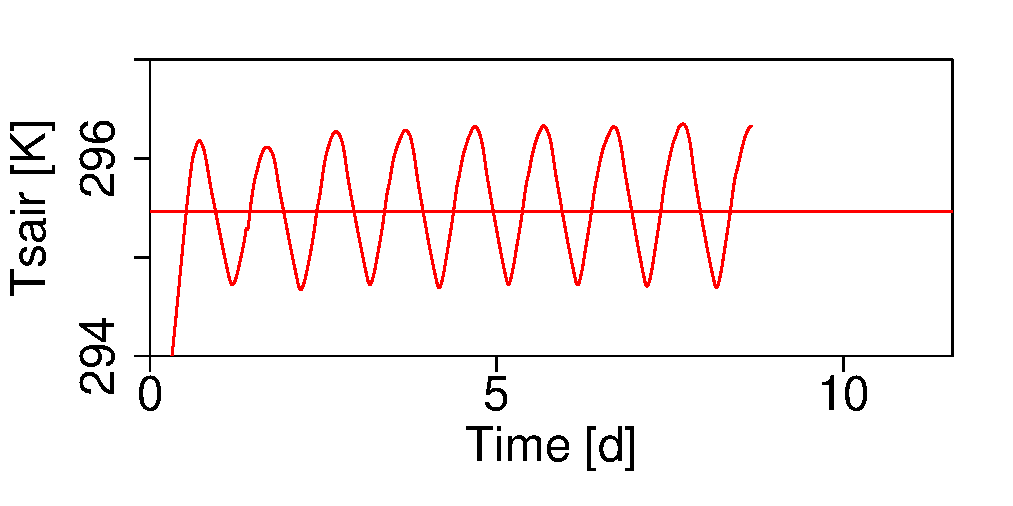
\includegraphics[trim={0 1.35cm 0cm 0}, clip, width=0.45\linewidth]{tsair_T0_300K_ampl_10_1km_timeseries.pdf}}
\put( 30,36){
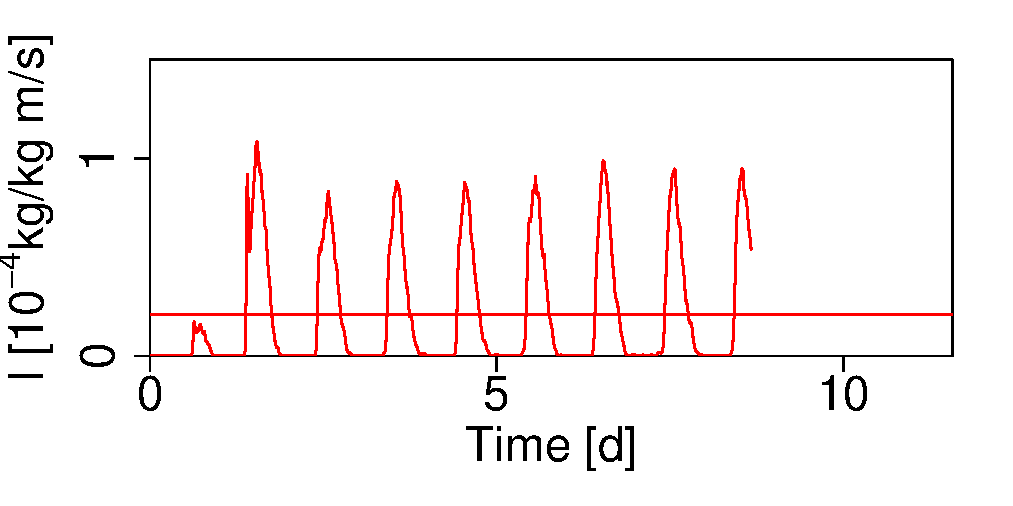
\includegraphics[trim={0 1.35cm 0cm 0}, clip, width=0.45\linewidth]{prcp_T0_300K_ampl_10_1km_timeseries.pdf}}
\put(-55,-1){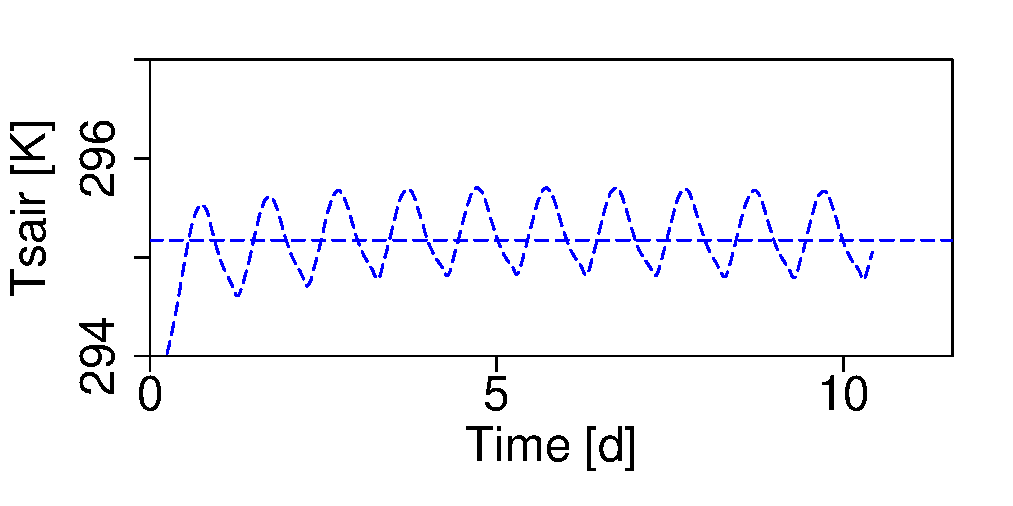
\includegraphics[trim={0 0cm 0cm 0}, clip, width=0.45\linewidth]{tsair_T0_300K_ampl_4_1km_timeseries.pdf}}
\put( 30,-1){
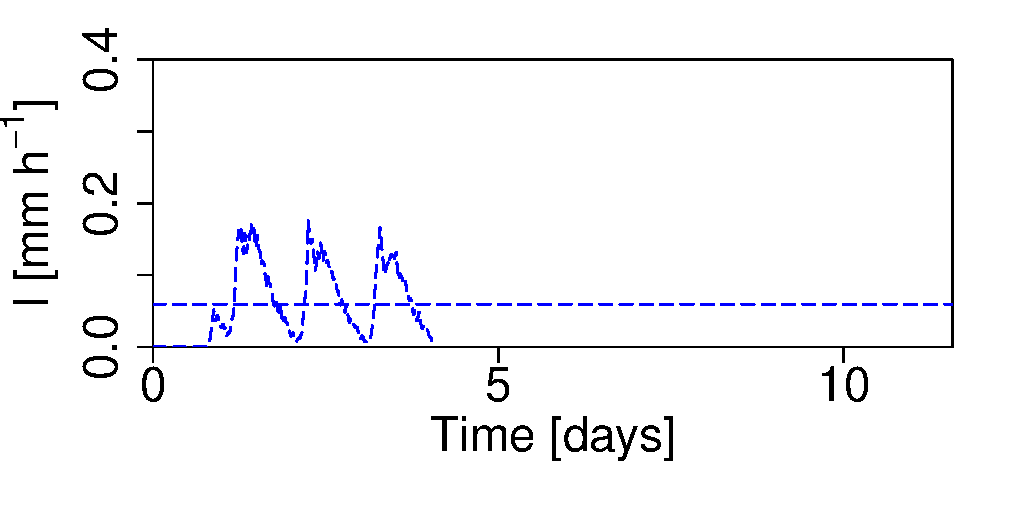
\includegraphics[trim={0 0 0cm 0}, clip, width=0.45\linewidth]{prcp_T0_300K_ampl_4_1km_timeseries.pdf}}
\put(-42,65){\bf a}
\put( 45,65){\bf b}
\put(-42,35){\bf c}
\put( 45,35){\bf d}
%\put( 62,53){\bf c}
\end{overpic}
\caption{{\bf Multi-day timeseries of domain averaged quantities}. 
{\bf a}, Domain-mean near-surface temperature for simulation A5b. The horizontal line indicates the time average over the entire time-series;
{\bf b}, Analogous to (a), but for rain rate;
{\bf c,d}, Analogous to (a),(b), but for the simulation A2b ({\it compare}: Tab.~\ref{tab:experiments}).}
\label{fig:multi-day_timeseries}
\end{figure*}

\begin{figure*}[ht]
\centering
\begin{overpic}[width=0.4\textwidth ]{dummy.pdf}
\put(-60,0){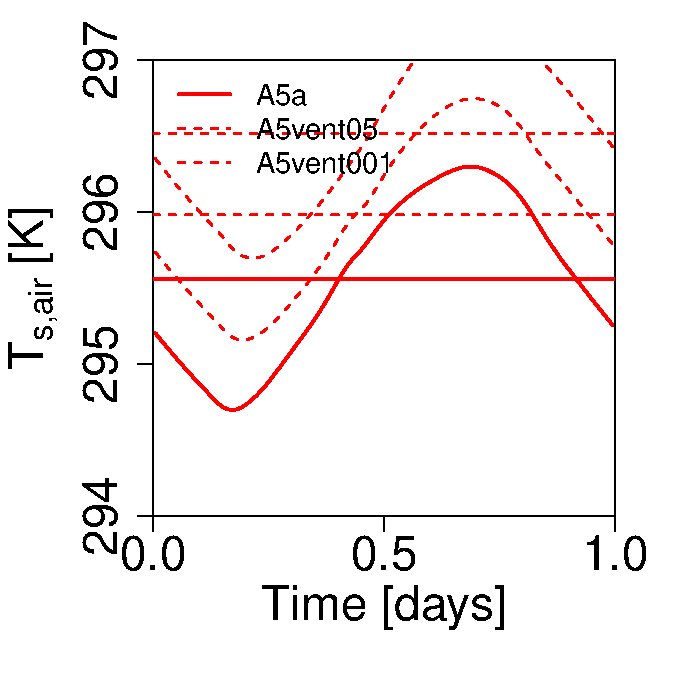
\includegraphics[trim={0 0 0cm 0}, clip, height=0.32\linewidth]{tsair_vent_timeseries_agg.pdf}}
\put(-5,0){
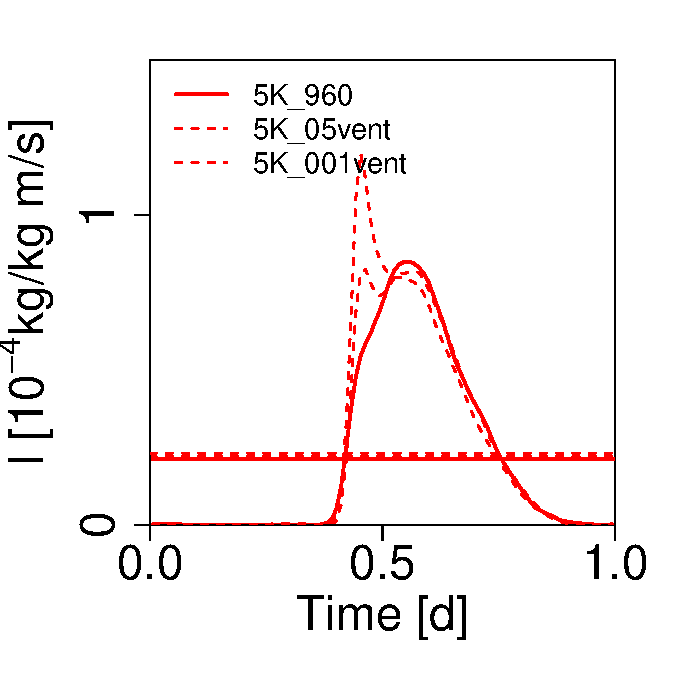
\includegraphics[trim={0 0 0cm 0}, clip, height=0.32\linewidth]{prcp_vent_timeseries_agg.pdf}}
\put(50,0){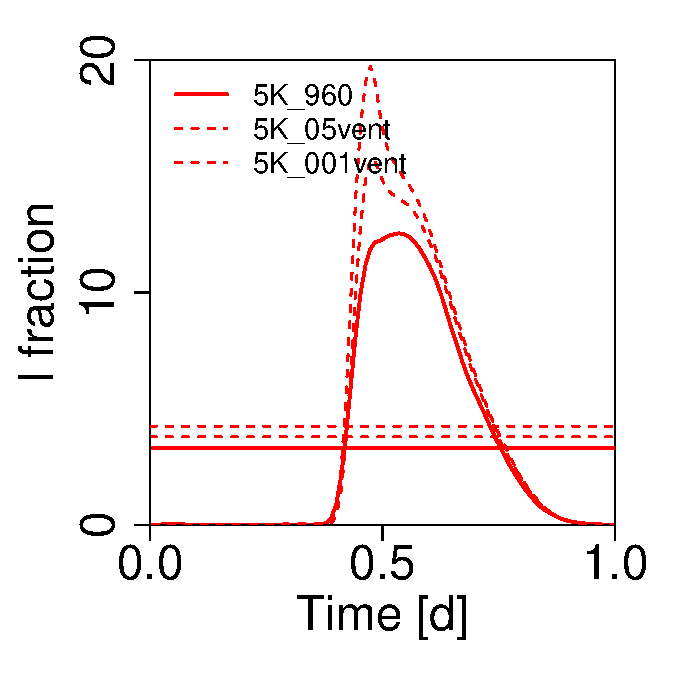
\includegraphics[trim={0 0 0cm 0}, clip, height=0.32\linewidth]{pfrac_vent_timeseries_agg.pdf}}
\put(-45,53){\bf a}
\put( 11,53){\bf b}
\put( 62,53){\bf c}
\end{overpic}
\caption{{\bf Diurnal cycles of domain averaged quantities}. 
%[here we might also want to show $T(6000m)$ and specific humidity.]
Similar to Fig.~\ref{fig:daily_mean} but reducing the ventilation coefficient \cite{seifert2006two} to a fraction of $.5$ and $.01$, respectively.
}
\label{fig:domain_mean_timeseries_ventilation}
\end{figure*}

\begin{figure*}[ht]
\centering
\begin{overpic}[width=0.4\textwidth ]{dummy.pdf}
\put(-60,0){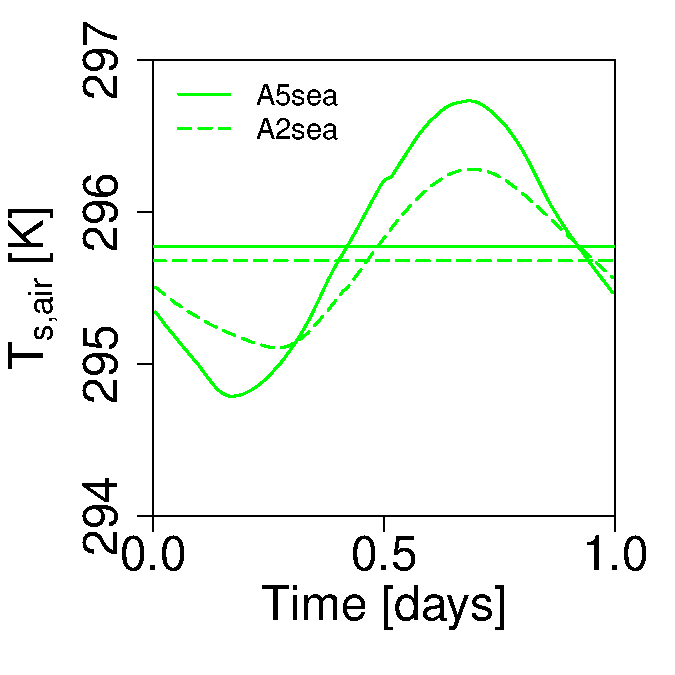
\includegraphics[trim={0 0 0cm 0}, clip, height=0.32\linewidth]{tsair_sea_timeseries_agg.pdf}}
\put(-5,0){
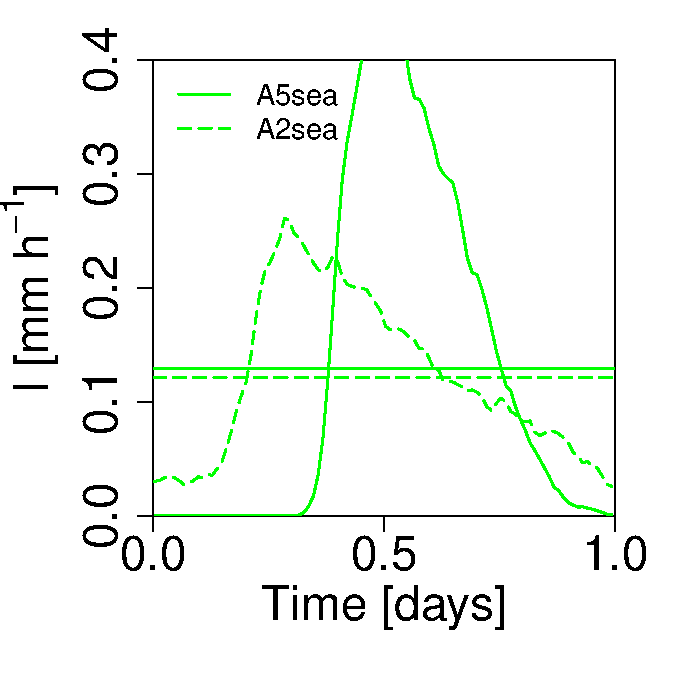
\includegraphics[trim={0 0 0cm 0}, clip, height=0.32\linewidth]{prcp_sea_timeseries_agg.pdf}}
\put(50,0){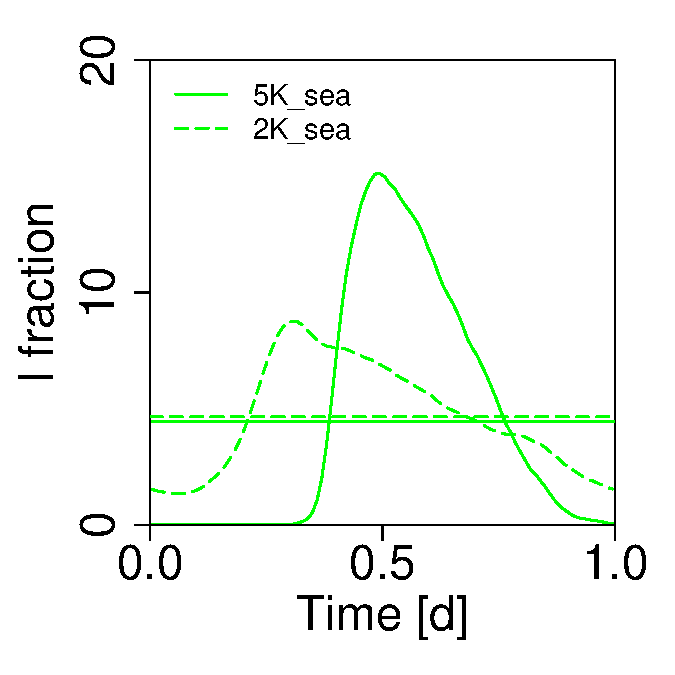
\includegraphics[trim={0 0 0cm 0}, clip, height=0.32\linewidth]{pfrac_sea_timeseries_agg.pdf}}
\put(-45,53){\bf a}
\put( 11,53){\bf b}
\put( 62,53){\bf c}
\end{overpic}
\caption{{\bf Diurnal cycles of domain averaged quantities}. 
%[here we might also want to show $T(6000m)$ and specific humidity.]
Similar to Fig.~\ref{fig:daily_mean} but using $100$ percent surface evaporation, mimicking a sea surface.
}
\label{fig:domain_mean_timeseries_surface_evap}
\end{figure*}

\begin{figure*}[ht]
\centering
%\begin{overpic}
%\includegraphics[height=0.33\linewidth]{cavities}
\centering
\begin{overpic}[width=0.4\textwidth ]{dummy.pdf}
\put(-55,0){
\includegraphics[trim={0 0 0cm 0}, clip, height=0.32\linewidth]{t_varying_ampl_timeseries_agg_p.pdf}}
\put(0,0){
\includegraphics[trim={0cm 0 0cm 0}, clip, height=0.32\linewidth]{t_sea_timeseries_agg_p.pdf}}
\put(55,0){\includegraphics[trim={0cm 0 0cm 0}, clip, height=0.32\linewidth]{t_vent_timeseries_agg_p.pdf}}
\put(-42,53){\bf a}
\put( 14,53){\bf b}
\put( 67,53){\bf c}
\end{overpic}
\caption{{\bf Diurnal cycles of surface and free troposphere temperature}. 
%[here we might also want to show $T(6000m)$ and specific humidity.]
[several things need correcting here]
As in Fig.~\ref{fig:daily_mean}a, but including free-tropospheric temperature [add the exact height when ready].
{\bf a}, Varying forcing amplitude $T_a$;
{\bf b}, Similar, but for sea surface conditions;
{\bf c}, Varying the ventilation coefficient.
}
\label{fig:free_trop_temp}
\end{figure*}

%\begin{figure*}[ht]
%\centering
%\centering
%\begin{overpic}[width=0.4\textwidth ]{dummy.pdf}
%\put(-55,0){
%\includegraphics[trim={0 0 0cm 0}, clip, height=0.32\linewidth]{q_varying_ampl_timeseries_agg_p.pdf}}
%\put(0,0){
%\includegraphics[trim={0cm 0 0cm 0}, clip, height=0.32\linewidth]{q_sea_timeseries_agg_p.pdf}}
%\put(55,0){\includegraphics[trim={0cm 0 0cm 0}, clip, height=0.32\linewidth]{q_vent_timeseries_agg_p.pdf}}
%\put(-42,53){\bf a}
%\put( 14,53){\bf b}
%\put( 67,53){\bf c}
%\end{overpic}
%\caption{{\bf Diurnal cycles of surface and free troposphere specific humidity}. 
%As in Fig.~\ref{fig:free_trop_temp}, but for free-tropospheric specific humidity [add the exact height when ready].
%}
%\label{fig:humidity}
%\end{figure*}

\begin{figure}[ht]
\centering
%\begin{overpic}
%\includegraphics[height=0.33\linewidth]{cavities}
\includegraphics[trim={2cm 2.4cm 1cm 1cm}, clip, height=0.11\linewidth]{var1_daymean_T0_300K_ampl_10_1km_large_1-144.png}
\includegraphics[trim={2cm 2.4cm 1cm 1cm}, clip, height=0.11\linewidth]{var1_daymean_T0_300K_ampl_10_1km_large_145-288.png}
\includegraphics[trim={2cm 2.4cm 1cm 1cm}, clip, height=0.11\linewidth]{var1_daymean_T0_300K_ampl_10_1km_large_289-432.png}
\includegraphics[trim={2cm 2.4cm 1cm 1cm}, clip, height=0.11\linewidth]{var1_daymean_T0_300K_ampl_10_1km_large_289-432.png}
\includegraphics[trim={2cm 2.4cm 1cm 1cm}, clip, height=0.11\linewidth]{var1_daymean_T0_300K_ampl_10_1km_large_433-576.png}
\includegraphics[trim={2cm 2.4cm 1cm 1cm}, clip, height=0.11\linewidth]{var1_daymean_T0_300K_ampl_10_1km_large_577-720.png}
\includegraphics[trim={2cm 2.4cm 1cm 1cm}, clip, height=0.11\linewidth]{var1_daymean_T0_300K_ampl_10_1km_large_721-846.png}\\
\includegraphics[trim={2cm 2.4cm 1cm 1cm}, clip, height=0.11\linewidth]{var1_daymean_T0_300K_ampl_4_1km_large_1-96.png}
\includegraphics[trim={2cm 2.4cm 1cm 1cm}, clip, height=0.11\linewidth]{var1_daymean_T0_300K_ampl_4_1km_large_289-384.png}
\includegraphics[trim={2cm 2.4cm 1cm 1cm}, clip, height=0.11\linewidth]{var1_daymean_T0_300K_ampl_4_1km_large_385-480.png}
\includegraphics[trim={2cm 2.4cm 1cm 1cm}, clip, height=0.11\linewidth]{var1_daymean_T0_300K_ampl_4_1km_large_481-576.png}
\includegraphics[trim={2cm 2.4cm 1cm 1cm}, clip, height=0.11\linewidth]{var1_daymean_T0_300K_ampl_4_1km_large_673-768.png}

\caption{{\bf Daily average precipitation intensity.} Similar to the heatmaps shown in Fig. \ref{fig:daily_mean} but for all available data. 
The top panels show $A5a$ for days 1---7, bottom panels show $A2a$ for days 1---4, and 6.}
\label{fig:daily_sum_1km_large_many_days}
\end{figure}

\begin{figure}[ht]
\centering
%\begin{overpic}
%\includegraphics[height=0.33\linewidth]{cavities}
\includegraphics[trim={2cm 2.4cm 1cm 1cm}, clip, height=0.11\linewidth]{var1_daymean_T0_300K_ampl_10_1km_1-288.png}
\includegraphics[trim={2cm 2.4cm 1cm 1cm}, clip, height=0.11\linewidth]{var1_daymean_T0_300K_ampl_10_1km_333-600.png}
\includegraphics[trim={2cm 2.4cm 1cm 1cm}, clip, height=0.11\linewidth]{var1_daymean_T0_300K_ampl_10_1km_909-1176.png}
\includegraphics[trim={2cm 2.4cm 1cm 1cm}, clip, height=0.11\linewidth]{var1_daymean_T0_300K_ampl_10_1km_1197-1464.png}
\includegraphics[trim={2cm 2.4cm 1cm 1cm}, clip, height=0.11\linewidth]{var1_daymean_T0_300K_ampl_10_1km_1485-1752.png}
\includegraphics[trim={2cm 2.4cm 1cm 1cm}, clip, height=0.11\linewidth]{var1_daymean_T0_300K_ampl_10_1km_1773-2040.png}
\includegraphics[trim={2cm 2.4cm 1cm 1cm}, clip, height=0.11\linewidth]{var1_daymean_T0_300K_ampl_10_1km_2061-2348.png}\\
\includegraphics[trim={2cm 2.4cm 1cm 1cm}, clip, height=0.11\linewidth]{var1_daymean_T0_300K_ampl_7_1km_289-576.png}
\includegraphics[trim={2cm 2.4cm 1cm 1cm}, clip, height=0.11\linewidth]{var1_daymean_T0_300K_ampl_7_1km_433-576.png}
\includegraphics[trim={2cm 2.4cm 1cm 1cm}, clip, height=0.11\linewidth]{var1_daymean_T0_300K_ampl_7_1km_577-720.png}\\
\includegraphics[trim={2cm 2.4cm 1cm 1cm}, clip, height=0.11\linewidth]{var1_daymean_T0_300K_ampl_4_1km_1-288.png}
\includegraphics[trim={2cm 2.4cm 1cm 1cm}, clip, height=0.11\linewidth]{var1_daymean_T0_300K_ampl_4_1km_289-576.png}
\includegraphics[trim={2cm 2.4cm 1cm 1cm}, clip, height=0.11\linewidth]{var1_daymean_T0_300K_ampl_4_1km_577-864.png}
\caption{{\bf Daily average precipitation intensity.} Similar to Fig.~\ref{fig:daily_sum_1km_large_many_days}, but for $(480\;km)^2$ domain area. 
The top panels show $A5b$ for days 1---7; the middle panels show $A3.5$ for days 2---4; the bottom panels show $A2b$ for days 1---3.}
\label{fig:daily_sum_1km_many_days}
\end{figure}

\begin{figure}[ht]
\centering
%\begin{overpic}
%\includegraphics[height=0.33\linewidth]{cavities}
\includegraphics[trim={2cm 2.4cm 1cm 1cm}, clip, height=0.11\linewidth]{var1_daymean_T0_300K_ampl_10_500m_1-288.png}
\includegraphics[trim={2cm 2.4cm 1cm 1cm}, clip, height=0.11\linewidth]{var1_daymean_T0_300K_ampl_10_500m_289-576.png}
\includegraphics[trim={2cm 2.4cm 1cm 1cm}, clip, height=0.11\linewidth]{var1_daymean_T0_300K_ampl_10_500m_577-864.png}\\
\includegraphics[trim={2cm 2.4cm 1cm 1cm}, clip, height=0.11\linewidth]{var1_daymean_T0_300K_ampl_10_200m_1-144.png}
\includegraphics[trim={2cm 2.4cm 1cm 1cm}, clip, height=0.11\linewidth]{var1_daymean_T0_300K_ampl_10_200m_145-288.png}
\includegraphics[trim={2cm 2.4cm 1cm 1cm}, clip, height=0.11\linewidth]{var1_daymean_T0_300K_ampl_10_200m_289-432.png}
\caption{{\bf Daily average precipitation intensity for higher resolution.} 
Horizontal resolution is increased to $500\;m$ (top row) and $200\;m$ (bottom row), the domain size is chosen as $192\;km\times 192$ $km$ and $240\;km\times 240$ $km$. The three panels show days 1---3.}
\label{fig:daily_sum_higher_res}
\end{figure}

\begin{figure}[ht]
\centering
%\begin{overpic}
%\includegraphics[height=0.33\linewidth]{cavities}
\includegraphics[trim={2cm 2.4cm 1cm 1cm}, clip, height=0.11\linewidth]{var1_daymean_T0_300K_ampl_10_1km_909-1176.png}
\includegraphics[trim={2cm 2.4cm 1cm 1cm}, clip, height=0.11\linewidth]{var1_daymean_T0_300K_ampl_10_1km_05vent_433-576.png}
\includegraphics[trim={2cm 2.4cm 1cm 1cm}, clip, height=0.11\linewidth]{var1_daymean_T0_300K_ampl_10_1km_001vent_433-576.png}
\caption{{\bf Daily average precipitation intensity for modified cold pools.}. 
Model day 4 as in A5b (left panel), and for ventilation coefficients reduced to $.5$ (middle panel) and $.01$ (right panel), respectively.}
\label{fig:daily_sum_vent}
\end{figure}

\begin{figure}[ht]
\centering
%\begin{overpic}
%\includegraphics[height=0.33\linewidth]{cavities}
\includegraphics[trim={2cm 2.4cm 1cm 1cm}, clip, height=0.11\linewidth]{var1_daymean_T0_300K_ampl_10_1km_p2K_865-1152.png}
\includegraphics[trim={2cm 2.4cm 1cm 1cm}, clip, height=0.11\linewidth]{var1_daymean_T0_300K_ampl_10_1km_p2K_2593-2880.png}
\\
\includegraphics[trim={2cm 2.4cm 1cm 1cm}, clip, height=0.11\linewidth]{var1_daymean_T0_300K_ampl_10_1km_RH100_1-144.png}
\includegraphics[trim={2cm 2.4cm 1cm 1cm}, clip, height=0.11\linewidth]{var1_daymean_T0_300K_ampl_10_1km_RH100_145-288.png}
\includegraphics[trim={2cm 2.4cm 1cm 1cm}, clip, height=0.11\linewidth]{var1_daymean_T0_300K_ampl_10_1km_RH100_289-432.png}
\includegraphics[trim={2cm 2.4cm 1cm 1cm}, clip, height=0.11\linewidth]{var1_daymean_T0_300K_ampl_10_1km_RH100_433-576.png}
\\
\includegraphics[trim={2cm 2.4cm 1cm 1cm}, clip, height=0.11\linewidth]{var1_daymean_T0_300K_ampl_4_1km_RH100_1-144.png}
\includegraphics[trim={2cm 2.4cm 1cm 1cm}, clip, height=0.11\linewidth]{var1_daymean_T0_300K_ampl_10_1km_RH100_1-144.png}
\includegraphics[trim={2cm 2.4cm 1cm 1cm}, clip, height=0.11\linewidth]{var1_daymean_T0_300K_ampl_4_1km_RH100_1153-1296.png}
\caption{{\bf Daily average precipitation intensity for increased surface temperature and increased surface moisture.} 
Resolution is maintained at $1\;km$ horizontally, the domain size is chosen as $480\;km\times 480$ $km$. The two top panels show days 4 and 8 for P2K at $T_a=5\;K$; 
the four central panels show days 1---4 for RH100 at $T_a=5\;K$;
the two bottom panels show days 1---4 for RH100 at $T_a=2\;K$.}
\label{fig:daily_mean_increased_T_q}
\end{figure}

\begin{figure}[ht]
\centering
\includegraphics[trim={0cm 0cm 0cm 0cm}, clip, height=0.27\linewidth]{var_5K_480_p2K.pdf}
\includegraphics[trim={0cm 0cm 0cm 0cm}, clip, height=0.27\linewidth]{{var_3.5K_480}.pdf}\\
\includegraphics[trim={0cm 0cm 0cm 0cm}, clip, height=0.27\linewidth]{var_5K_05vent.pdf}
\includegraphics[trim={0cm 0cm 0cm 0cm}, clip, height=0.27\linewidth]{var_5K_001vent.pdf}\\
\includegraphics[trim={0cm 0cm 0cm 0cm}, clip, height=0.27\linewidth]{var_5K_480_500m.pdf}
\includegraphics[trim={0cm 0cm 0cm 0cm}, clip, height=0.27\linewidth]{var_5K_200m.pdf}\\
\includegraphics[trim={0cm 0cm 0cm 0cm}, clip, height=0.27\linewidth]{var_5K_sea.pdf}
\includegraphics[trim={0cm 0cm 0cm 0cm}, clip, height=0.27\linewidth]{var_2K_sea.pdf}
\caption{{\bf Normalized variance for further simulations.}
P2K with $T_a=5\;K$, reduced ventilation coefficients ($.5$ and $.01$ of the default values), $500\;m$ and $200\;m$ resolution with $T_a=5\;K$, sea surface with $T_a=5\;K$ and $T_a=2\;K$.
}
\label{fig:variance_further_sims}
\end{figure}

\begin{figure}[ht]
\centering
\begin{overpic}[width=0.4\textwidth]{dummy.pdf}
\put(-35,0){\includegraphics[trim={0cm 0cm 0cm 0cm}, clip, height=0.37\linewidth]{T0_300K_ampl_4_1km_865-1172_hist_CP_Height.pdf}}
\put(20,0){\includegraphics[trim={0cm 0cm 0cm 0cm}, clip, height=0.37\linewidth]{T0_300K_ampl_10_1km_909-1176_hist_CP_Height.pdf}}

\put(-30,59){\bf a}
\put(25,59){\bf b}
\end{overpic}
\vspace{0cm}
\caption{{\bf Cold Pool Height Distribution Functions.}
{\bf a}, Cold pool height distribution function for day four of A2b ({\it compare}: Fig.~\ref{fig:CP_merging}d). 
Each curve shows the histogram for all cold pool heights within five model timesteps (right vertical axis), that is, $480\times 480\times 5$ individual height values. 
A dominant peak occurs at zero height, which is not shown, as it correspondings to regions without cold pools.
The probability origin of each curve is shifted and marked by a grey horizontal line.  
{\bf b}, Analogous to (a), but for A5b during day four ({\it compare}: Fig.~\ref{fig:CP_merging}g).
Note the pronounced double-peak structure that emerges for A5b near mid-day.
}
\label{fig:CP_height_distribution}
\end{figure}


\begin{figure}[ht]
\centering
\includegraphics[]{T0_300K_ampl_10_1km_}
\vspace{0cm}
\caption{{\bf Cold Pool Height Distribution Functions.}
{\bf a}, Cold pool height distribution function for day four of A2b ({\it compare}: Fig.~\ref{fig:CP_merging}d). 
Each curve shows the histogram for all cold pool heights within five model timesteps (right vertical axis), that is, $480\times 480\times 5$ individual height values. 
A dominant peak occurs at zero height, which is not shown, as it correspondings to regions without cold pools.
The probability origin of each curve is shifted and marked by a grey horizontal line.  
{\bf b}, Analogous to (a), but for A5b during day four ({\it compare}: Fig.~\ref{fig:CP_merging}g).
Note the pronounced double-peak structure that emerges for A5b near mid-day.
}
\label{fig:CP_height_distribution}
\end{figure}


\begin{figure}[ht]
\centering
\begin{overpic}[width=0.4\textwidth]{dummy.pdf}
\put(-55,16){\includegraphics[trim={0cm 2.1cm 0cm 0cm}, clip, height=0.19\linewidth]{T0_300K_ampl_4_1km_865-11722dPlot_precip_marked_points.pdf}}
\put(-14,16){\includegraphics[trim={0cm 2.1cm 0cm 0cm}, clip, height=0.19\linewidth]{T0_300K_ampl_4_1km_865-1172_comparison_q_1.pdf}}
\put(10,16){\includegraphics[trim={2cm 2.1cm 0cm 0cm}, clip, height=0.19\linewidth]{T0_300K_ampl_4_1km_865-1172_comparison_q_277.pdf}}
\put(-55,-27.0){\includegraphics[trim={0cm 0cm 0cm 0cm}, clip, height=0.225\linewidth]{T0_300K_ampl_10_1km_909-11762dPlot_precip_marked_points.pdf}}
\put(-14,-28){\includegraphics[trim={0cm 0cm 0cm 0cm}, clip, height=0.23\linewidth]{T0_300K_ampl_10_1km_909-1176_comparison_q_17.pdf}}
\put(10,-28){\includegraphics[trim={2cm 0cm 0cm 0cm}, clip, height=0.23\linewidth]{T0_300K_ampl_10_1km_909-1176_comparison_q_221.pdf}}

\put(-48,49){\bf a}
\put(-6,49){\bf b}
\put(11,49){\bf c}
\put(-48,12){\bf d}
\put(-6,12){\bf e}
\put(11,12){\bf f}
%\put(-45,72){\large $\Delta T=5\;K$}
%\put(-45,25){\large $\Delta T=2\;K$}
\end{overpic}
\vspace{2cm}
\caption{{\bf Moisture oscillations.}
{\bf a}, Simulation $A2b$ day four. Spatial rain distribution (red) with high and low values marked in light blue circles and green diamonds, respectively. 
{\bf b}, Specific humidity vs height for intense and weak precipitation regions before the onset of precipitation (early morning).
{\bf c}, Analogous to (b), but at the end of the model day.
{\bf d---f}, Analogous to (a)---(c), but for $A5b$.
Note the moisture oscillations and the logarithmic vertical axis scaling in panels b,c,e,f.
}
\label{fig:moisture_oscillations}
\end{figure}

\begin{figure}[ht]
\centering
\begin{overpic}[width=0.4\textwidth ]{dummy.pdf}
\put(-20,0){\includegraphics[height=0.57\linewidth,trim=0cm 0cm 0cm 0cm, clip]{variance_scan.pdf}}
\end{overpic}
\caption{{\bf Variance as a function of density for simple checkerboard model.}
The plot shows several different values of linear system size ($N$) as marked in legend.
Each point represents the steady-state value of normalized variance for one realization of the system, starting with random initial conditions, where each sub-domain of $L^2=20\times 20$ sites were populated by filling each grid point at probability $p_0$.
The black dashed line represents the variance obtainable for a checkerboard pattern with $N^2/2$ lattice sites (half of them) containing $2p_0L^2$, hence all the available points, and $N^2/2$ lattice sites (the other half) containing zero points.
}
\label{fig:variance_vs_density}
\end{figure}

\begin{figure*}[ht]
\centering
\begin{overpic}[width=0.4\textwidth ]{dummy.pdf}
\put(-70,40){\includegraphics[height=0.37\linewidth,trim=0cm 2cm 0cm 0cm, clip]{{Ta=0.10_N=960day_1}.png}}
\put(0,40){\includegraphics[trim={2.5cm 2cm 0cm 0cm}, clip, height=0.37\linewidth½]{{Ta=0.10_N=960day_6}.png}}
\put(60,40){\includegraphics[trim={2.5cm 2cm 0cm 0cm}, clip, height=0.37\linewidth]{{Ta=0.10_N=960day_7}.png}}
\put(-70,-35){\includegraphics[trim={0cm 0cm 0cm 0cm}, clip, height=0.42\linewidth]{{Ta=0.50_N=960day_1}.png}}
\put(0,-35){\includegraphics[trim={2.5cm 0cm 0cm 0cm}, clip, height=0.42\linewidth]{{Ta=0.50_N=960day_6}.png}}
\put(60,-35){\includegraphics[trim={2.5cm 0cm 0cm 0cm}, clip, height=0.42\linewidth]{{Ta=0.50_N=960day_7}.png}}
\put(-58,102){\large \bf a}
\put(-0,102){\large \bf b}
\put(62,102){\large \bf c}
\put(-58,36){\large \bf d}
\put(-0,36){\large \bf e}
\put(62,36){\large \bf f}

\put(-58,90){\large small $T_a$}
\put(-58,27){\large large $T_a$}

\put(10,77){\color{black}\line(0,-0.5){5}}
\put(10,72){\color{black}\line(.5,0){5}}
\put(10,77){\color{black}\line(.5,0){5}}
\put(15,77){\color{black}\line(0,-0.5){5}}

\put(10,10){\color{black}\line(0,-1){5}}
\put(10,5){\color{black}\line(1,0){5}}
\put(10,10){\color{black}\line(1,0){5}}
\put(15,10){\color{black}\line(0,-1){5}}

\put(70,77){\color{black}\line(0,-1){5}}
\put(70,72){\color{black}\line(1,0){5}}
\put(70,77){\color{black}\line(1,0){5}}
\put(75,77){\color{black}\line(0,-1){5}}

\put(70,10){\color{black}\line(0,-1){5}}
\put(70,5){\color{black}\line(1,0){5}}
\put(70,10){\color{black}\line(1,0){5}}
\put(75,10){\color{black}\line(0,-1){5}}

\end{overpic}
%\begin{picture}
%\put(0,15){\circle(20)}
%\end{picture}
\vspace{2.2cm}
\caption{{\bf Transition to a clustered rainfall state in the simplified model.}
{\bf a}, Surface rainfall average during the first day ($t=1\;d$, spin up) for $\Delta T=2\;K$.
{\bf b}, Similar to (a), but for $t=6\;d$.
{\bf c}, Similar to (a), but for $t=7\;d$.
{\bf d---f}, Similar to (a)---(c), but for large amplitude.
To highlight the spatial and temporal variation, boxes of side length $l=150\;km$ are shown at equal positions in panels b,c,e,f.
Pixels in white, blue and green correspond to zero, one, or two rain events, occurring within the respective model day.
}
\label{fig:daily_mean_simplified_model}
\end{figure*}

\end{document}